\section{Астатизм нулевого порядка}
Рассмотрим замкнутую системы с объектом управления, описываемым передаточной функцией:
\begin{equation}
    W(s) = \frac{3}{s^2 + 7.5s + 2}
\end{equation}
И регулятором, описываемым передаточной функцией:
\begin{equation}
   H(s) = k
\end{equation}
Запишем передаточную функцию замкнутой системы:
\begin{equation}
    W_{u\rightarrow y}(s) = \frac{W(s)H(s)}{1 + W(s)H(s)} = \frac{3k}{s^2 + 7.5s + 2 + 3k}
\end{equation}
Согласно следствию из критерия Гурвица для систем второго порядка, система будет устойчива при:
\begin{equation}
    \begin{cases}
        7.5 > 0 \\ 
        2 + 3k > 0 \\ 
    \end{cases}
    \Rightarrow
    k > -\frac{2}{3} \\ 
\end{equation}
Найдем передаточную функцию по ошибке:
\begin{equation}
    W_{u\rightarrow e}(s) = \frac{1}{1 + W(s)H(s)} = \frac{s^2 + 7.5s + 2}{s^2 + 7.5s + 2 + 3k}
\end{equation}

\subsection{Статическая система}
Найдем образ Лапласа входного воздействия:
\begin{equation}
    L\{A\} = \frac{A}{s}
\end{equation}
Теперь найдем образ Лапласа выходного сигнала:
\begin{equation}
    Y = W_{u\rightarrow y}(s)L\{A\} = \frac{3k}{s^2 + 7.5s + 2 + 3k}\frac{A}{s} = \frac{3kA}{s(s^2 + 7.5s + 2 + 3k)}
\end{equation}
$sY$ не имеет положительных полюсов, следовательно, система устойчива. Теперь найдем установившееся значение ошибки, 
согласное теореме о конечном значении:
\begin{equation}
    E = W_{u\rightarrow e}(s)L\{A\} = \frac{s^2 + 7.5s + 2}{s^2 + 7.5s + 2 + 3k}\frac{A}{s} 
\end{equation}

\begin{equation}
    e_{\text{set}} = \lim_{s \to 0} sY = \lim_{s \to 0} \frac{A(s^2 + 7.5s + 2)}{s^2 + 7.5s + 2 + 3k} = \frac{2A}{2 + 3k}
\end{equation}

Промоделируем систему, представленную на рис. \ref{fig:task3_scheme}.
\begin{figure}[ht!]
    \centering
    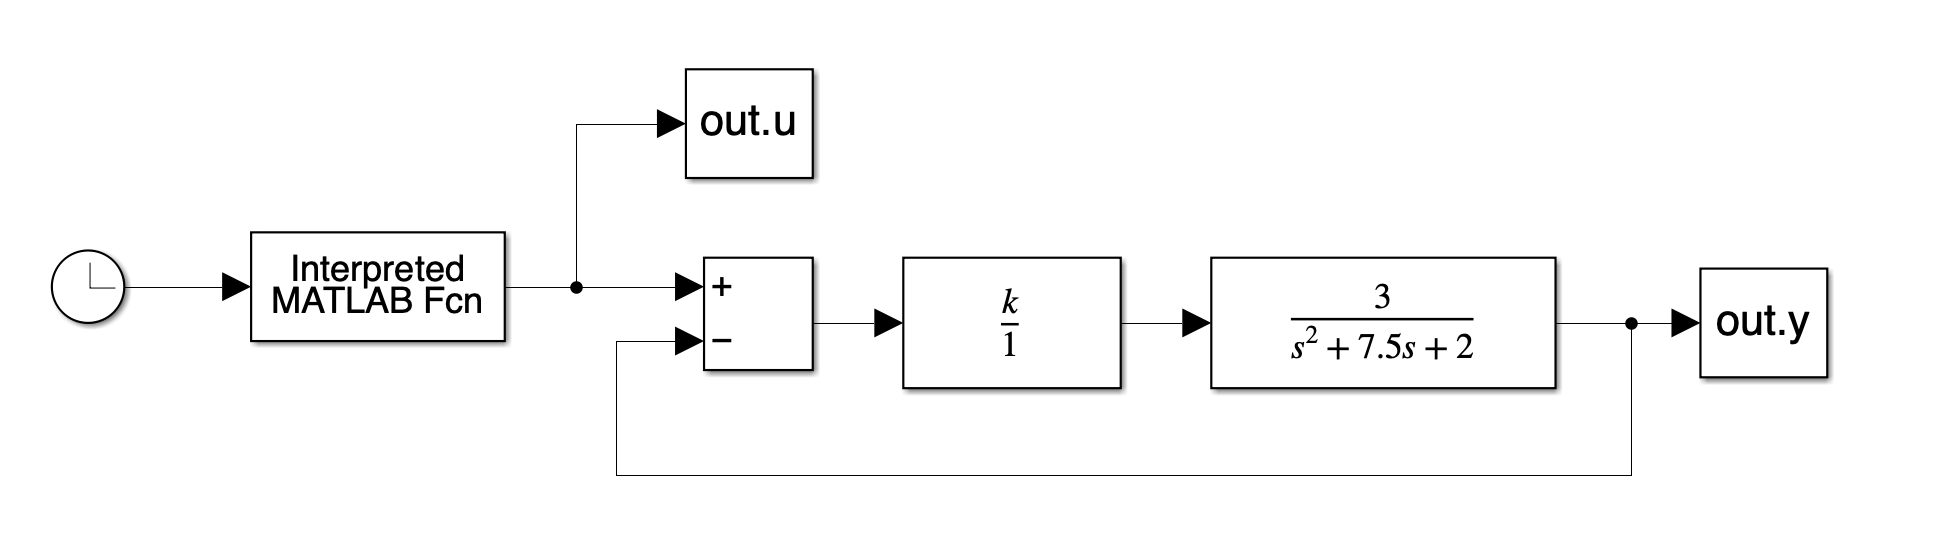
\includegraphics[width=\textwidth]{"media/scheme3.png"}
    \caption{Схема моделирования системы}
    \label{fig:task3_scheme}
\end{figure}

Результаты моделирования приведены на рис. \ref{fig:task3_out1}, \ref{fig:task3_error1}.

\begin{table}
    \centering
    \begin{tabular}{|c|c|c|}
        \hline
        $k$ & $e_{\text{set}}$ & $e_{\text{fact}}$ \\
        \hline
        -0.1 & 2.35 & 2.31 \\
        0.1 & 1.73 & 1.75 \\
        1 & 0.8 & 0.8 \\
        10 & 0.125 & 0.125 \\
        \hline
    \end{tabular}
    \caption{Сравнение теоретического и фактического установившегося значения ошибки}
\end{table}

\begin{figure}
    \centering
    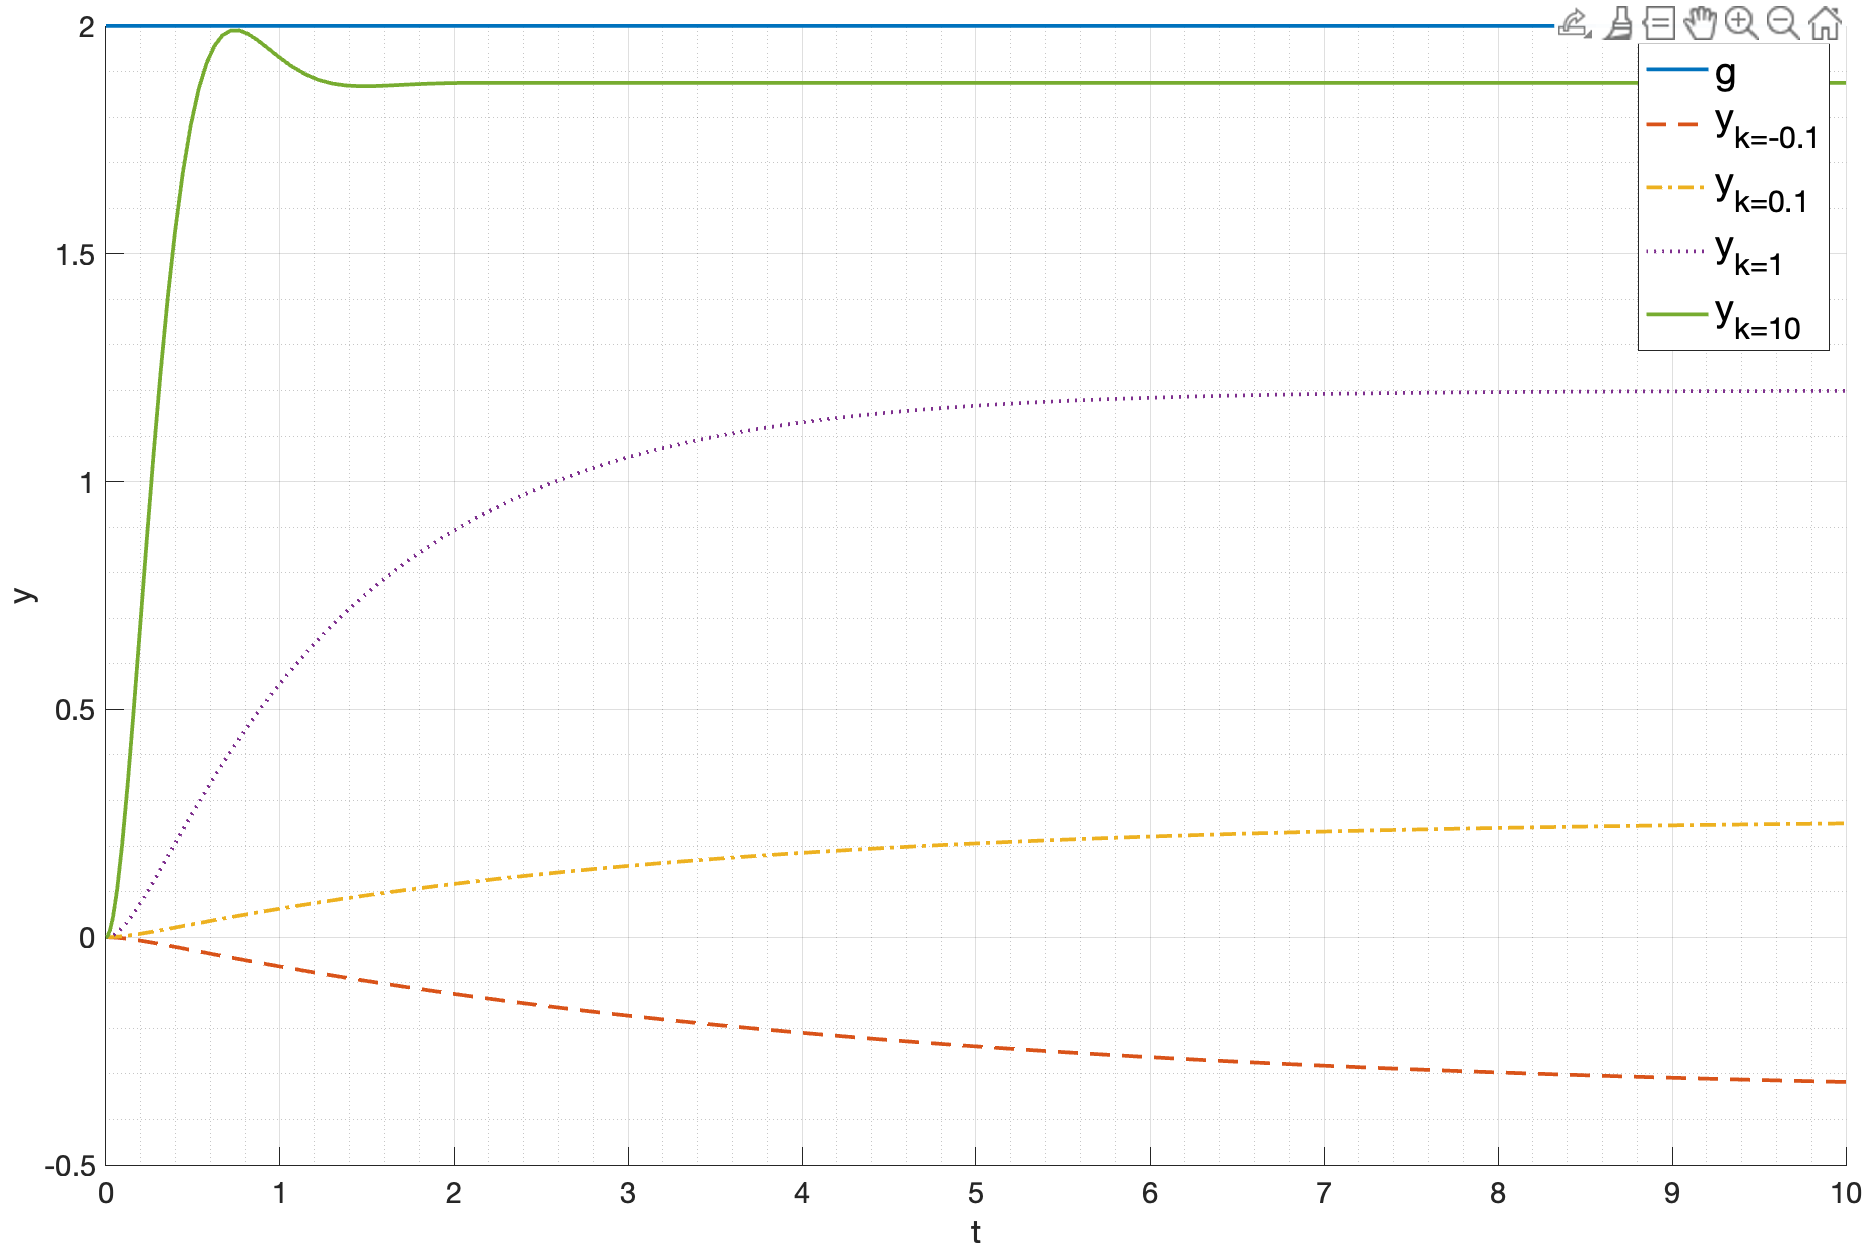
\includegraphics[width=\textwidth]{"media/plots/task3_out1.png"}
    \caption{Моделирование системы с P регулятором ($u(t) = A$)}
    \label{fig:task3_out1}
\end{figure}

\begin{figure}
    \centering
    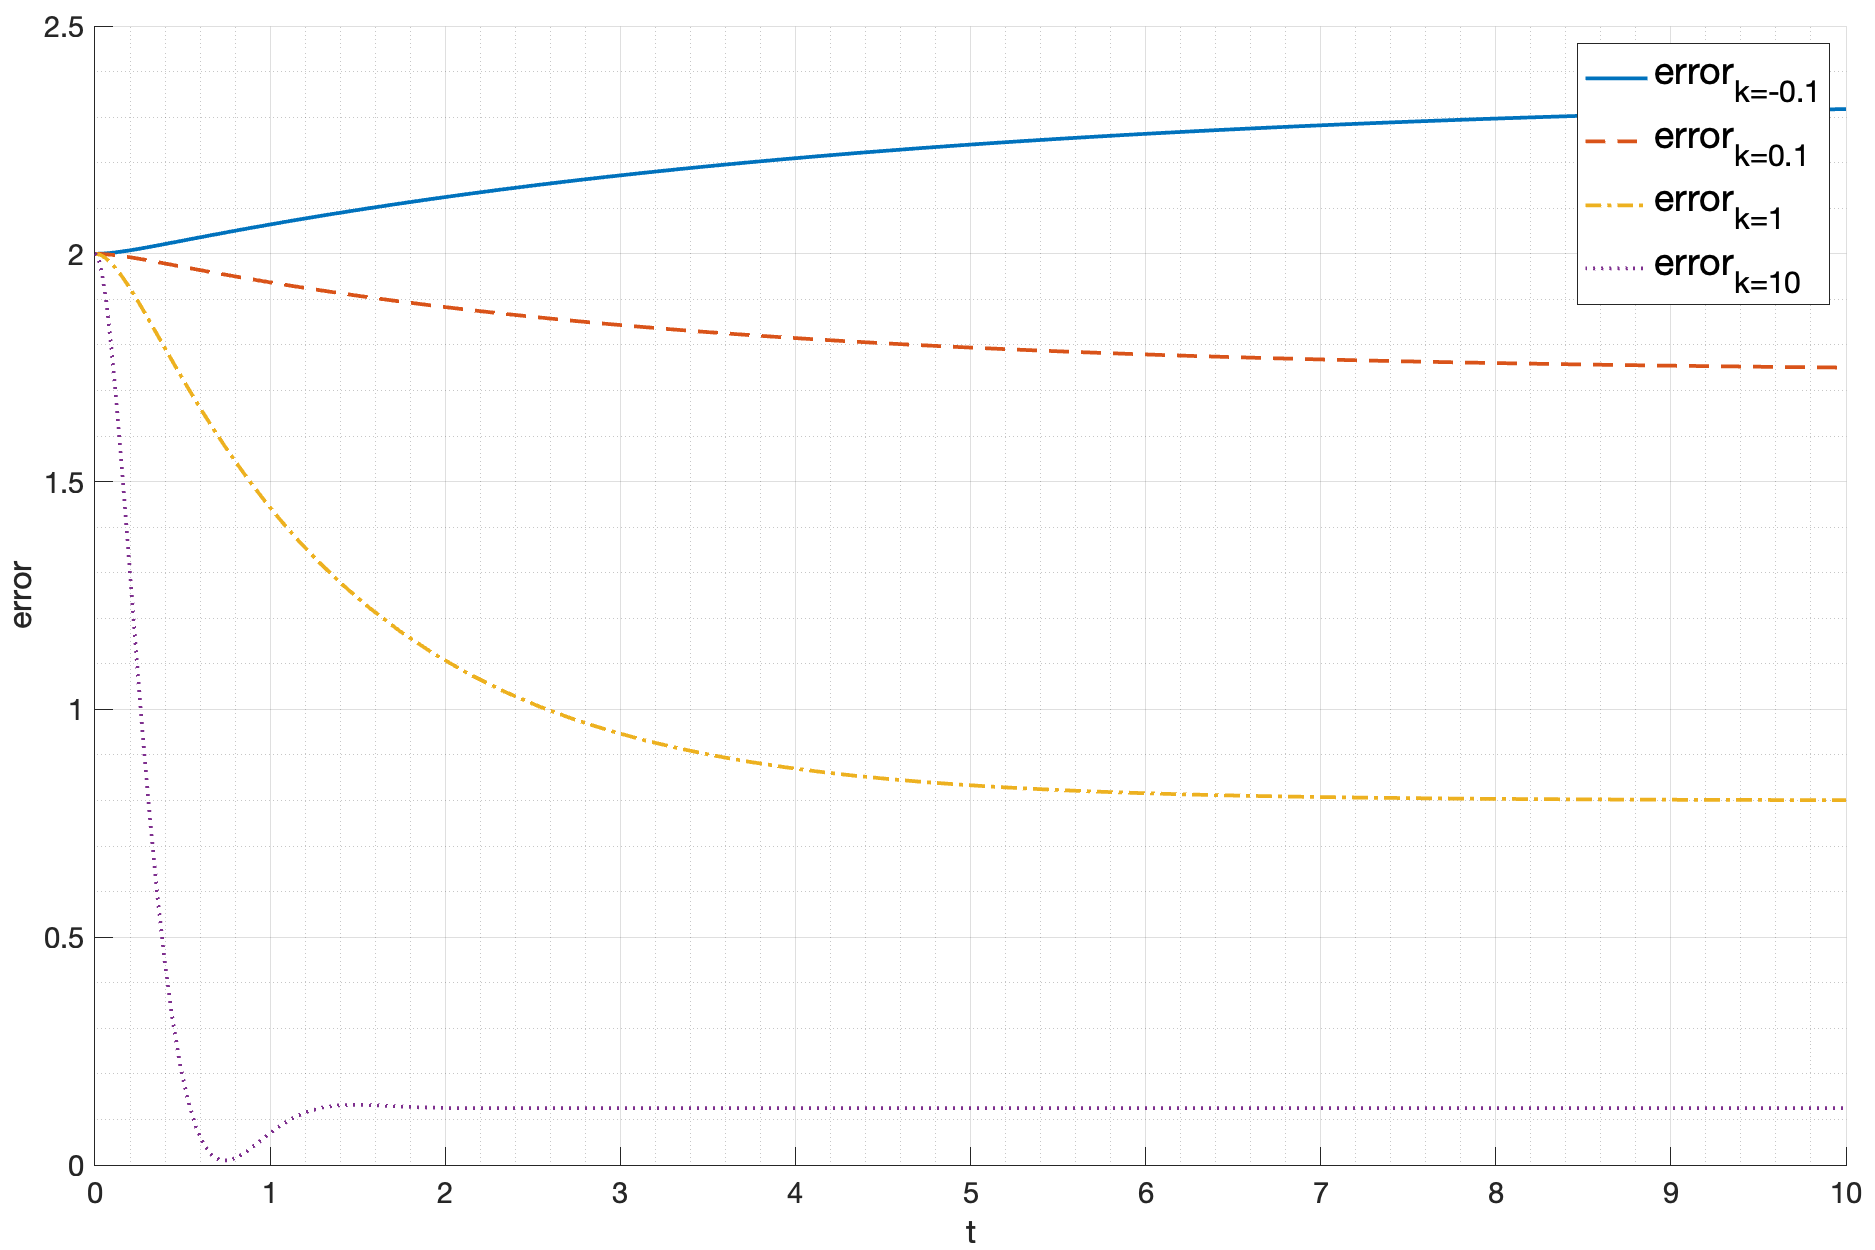
\includegraphics[width=\textwidth]{"media/plots/task3_error1.png"}
    \caption{График ошибки системы с P регулятором ($u(t) = A$)}
    \label{fig:task3_error1}
\end{figure}



% Возьмем $k = -0.1$. Таким образом, согласно теоретическим расчетам, система будет устойчива. Промоделируем (см рис. \ref{fig:task3_out}).
% Теоретическое значение установившегося значения ошибки: $e_{\text{set}} = \frac{2A}{2 + 3k} = 2.35$.
% \begin{figure}
%     \centering
%     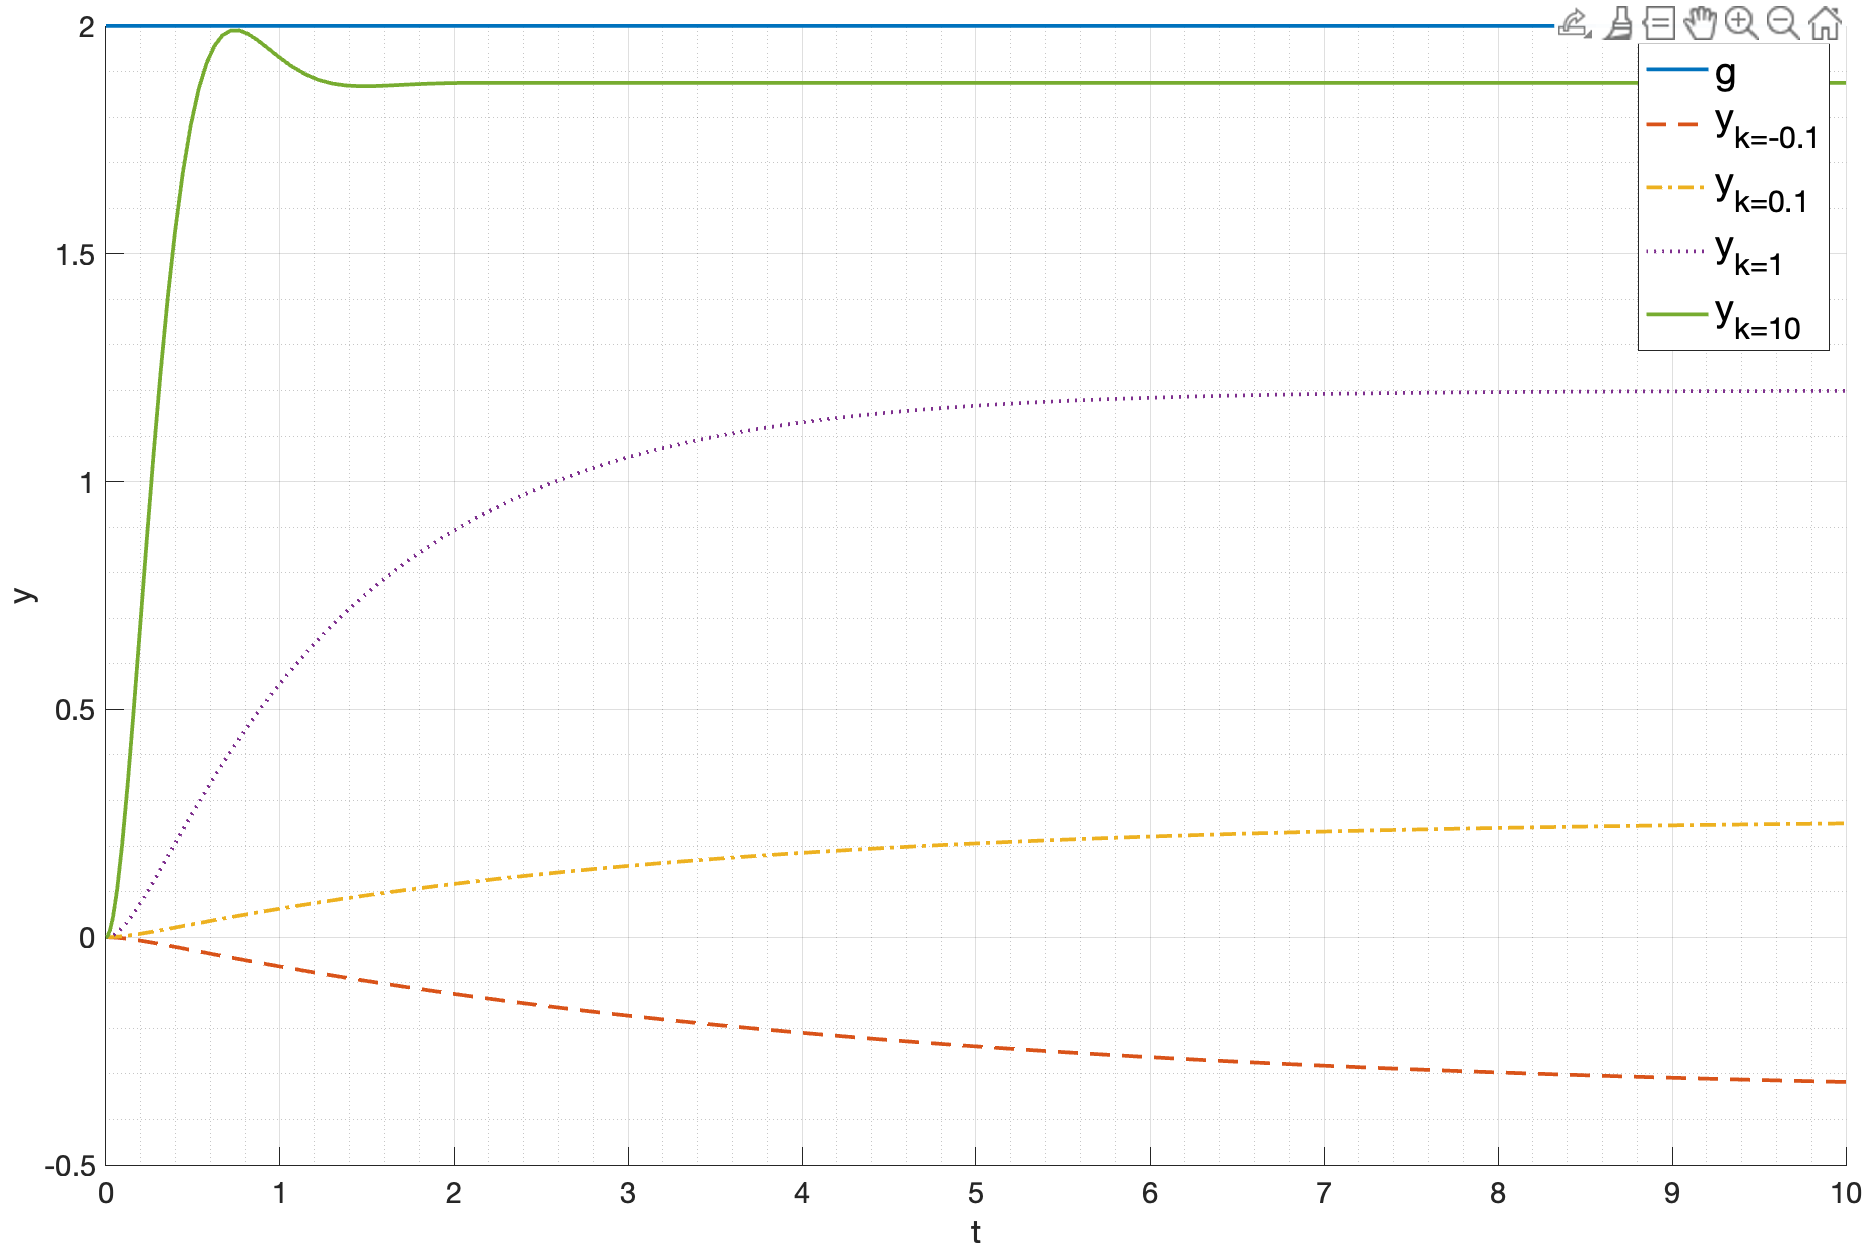
\includegraphics[width=\textwidth]{"media/plots/task3_out.png"}
%     \caption{Моделирование системы с P регулятором ($k = -0.1$) ($u(t) = A$)}
%     \label{fig:task3_out}
% \end{figure}
% Фактическое значение установившегося значения ошибки  $e_{\text{fact}} = 2.31$.

% Возьмем $k = 0.1$. Промоделируем (см рис. \ref{fig:task3_out2}).
% Теоретическое значение установившегося значения ошибки: $e_{\text{set}} = \frac{2A}{2 + 3k} = 1.73$.
% \begin{figure}
%     \centering
%     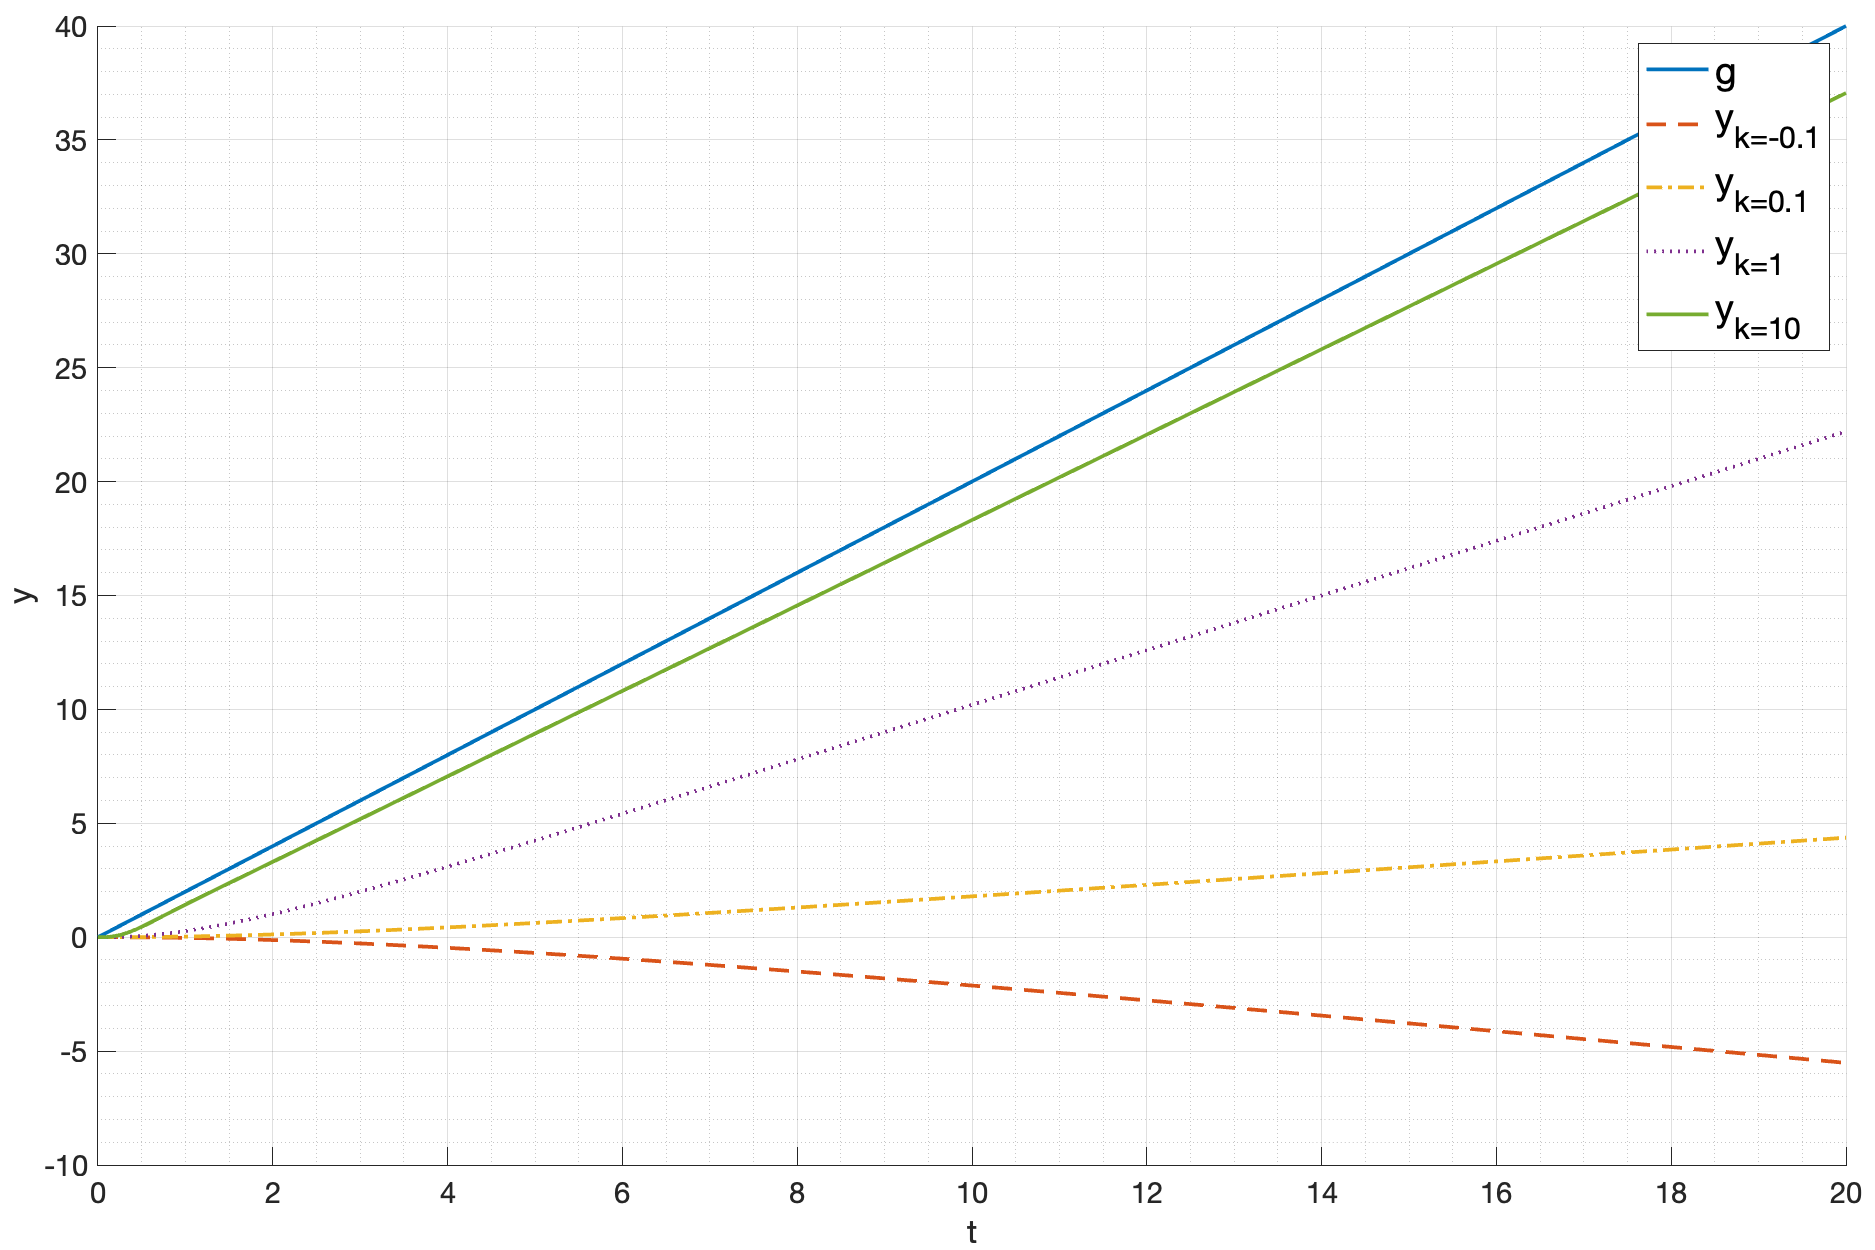
\includegraphics[width=\textwidth]{"media/plots/task3_out2.png"}
%     \caption{Моделирование системы с P регулятором ($k = 0.1$) ($u(t) = A$)}
%     \label{fig:task3_out2}
% \end{figure}
% Фактическое значение установившегося значения ошибки  $e_{\text{fact}} = 1.75$.

% Возьмем $k = 1$. Промоделируем (см рис. \ref{fig:task3_out3}).
% Теоретическое значение установившегося значения ошибки: $e_{\text{set}} = \frac{2A}{2 + 3k} = 0.8$.
% \begin{figure}
%     \centering
%     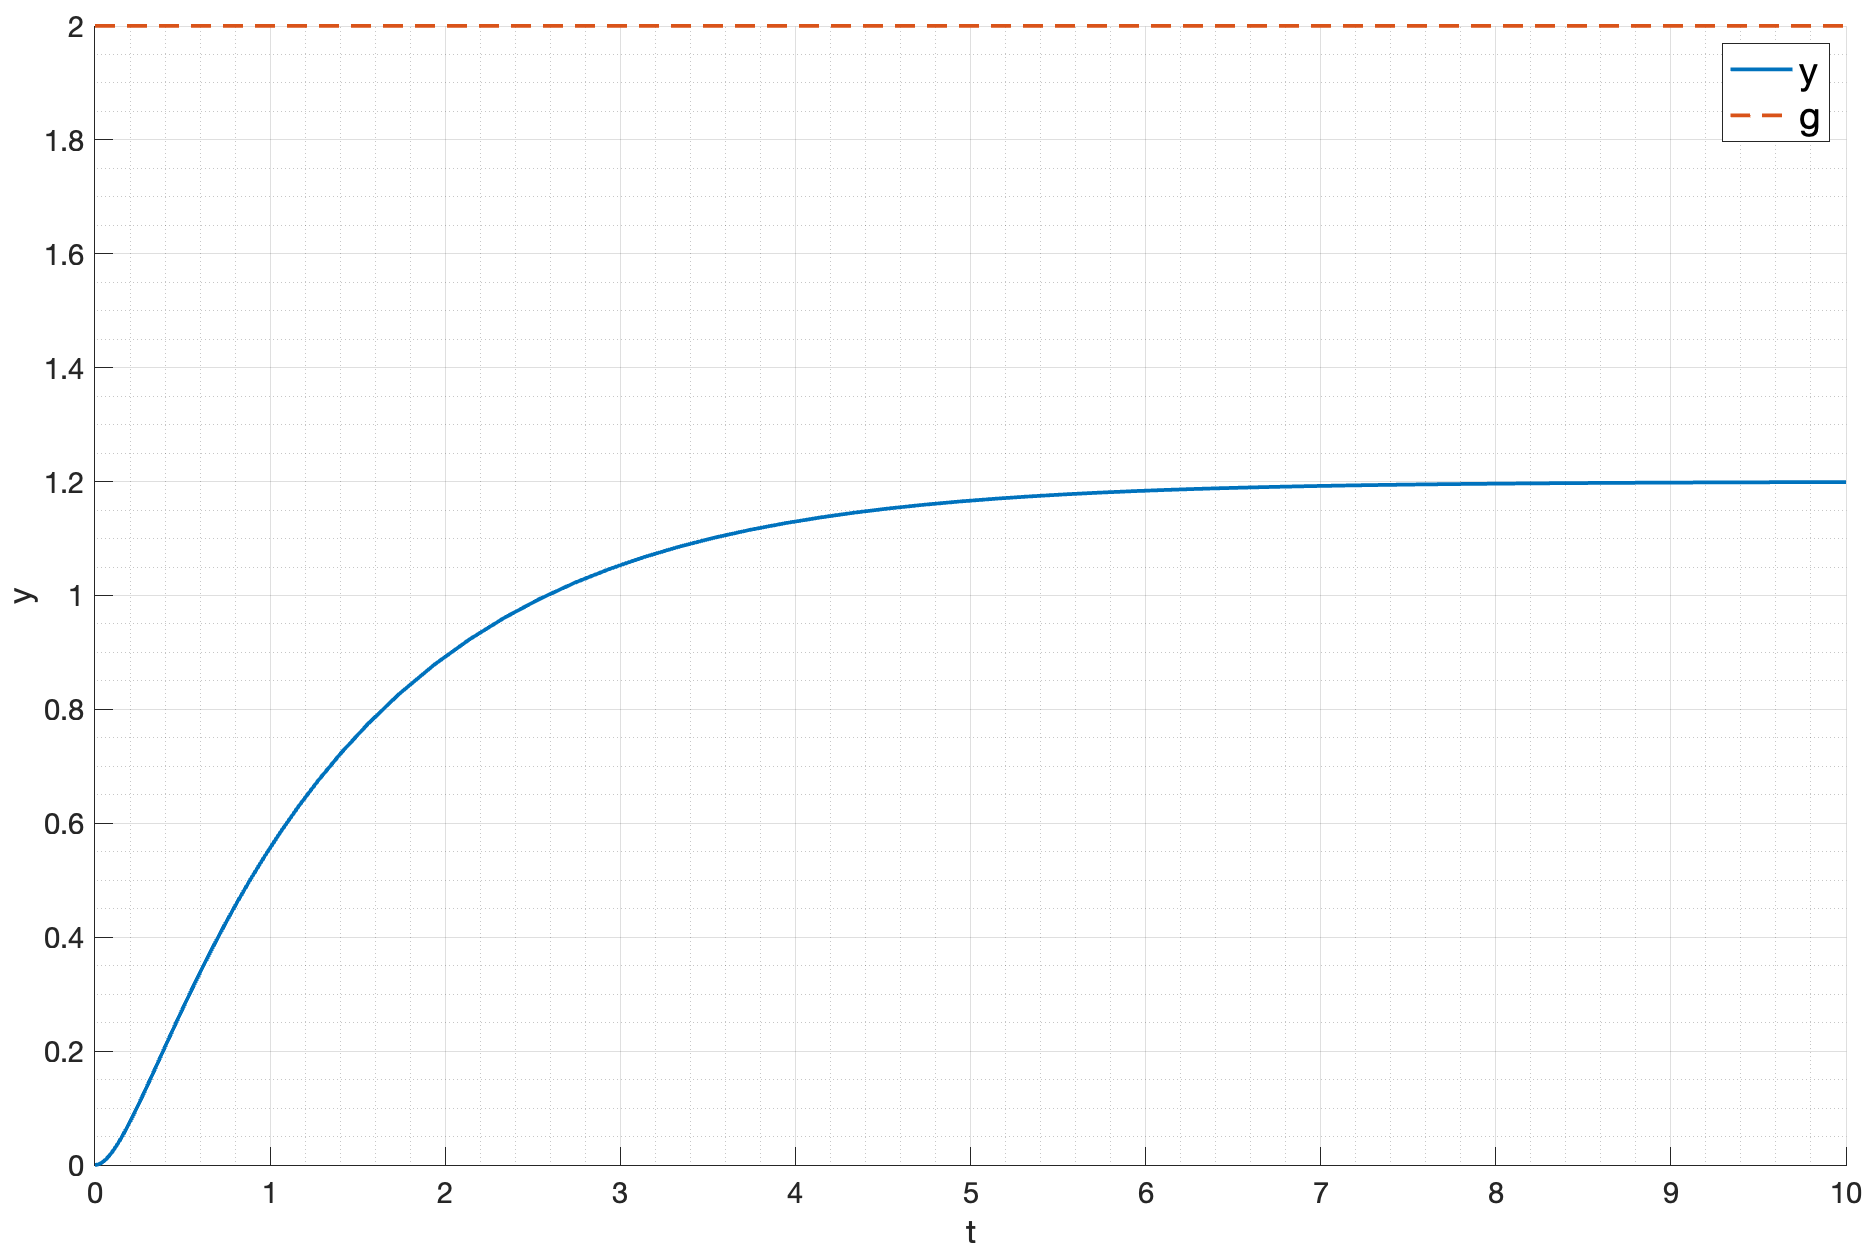
\includegraphics[width=\textwidth]{"media/plots/task3_out3.png"}
%     \caption{Моделирование системы с P регулятором ($k = 1$) ($u(t) = A$)}
%     \label{fig:task3_out3}
% \end{figure}
% Фактическое значение установившегося значения ошибки  $e_{\text{fact}} = 0.8$.

% Возьмем $k = 10$. Промоделируем (см рис. \ref{fig:task3_out4}).
% Теоретическое значение установившегося значения ошибки: $e_{\text{set}} = \frac{2A}{2 + 3k} = 0.125$.
% \begin{figure}
%     \centering
%     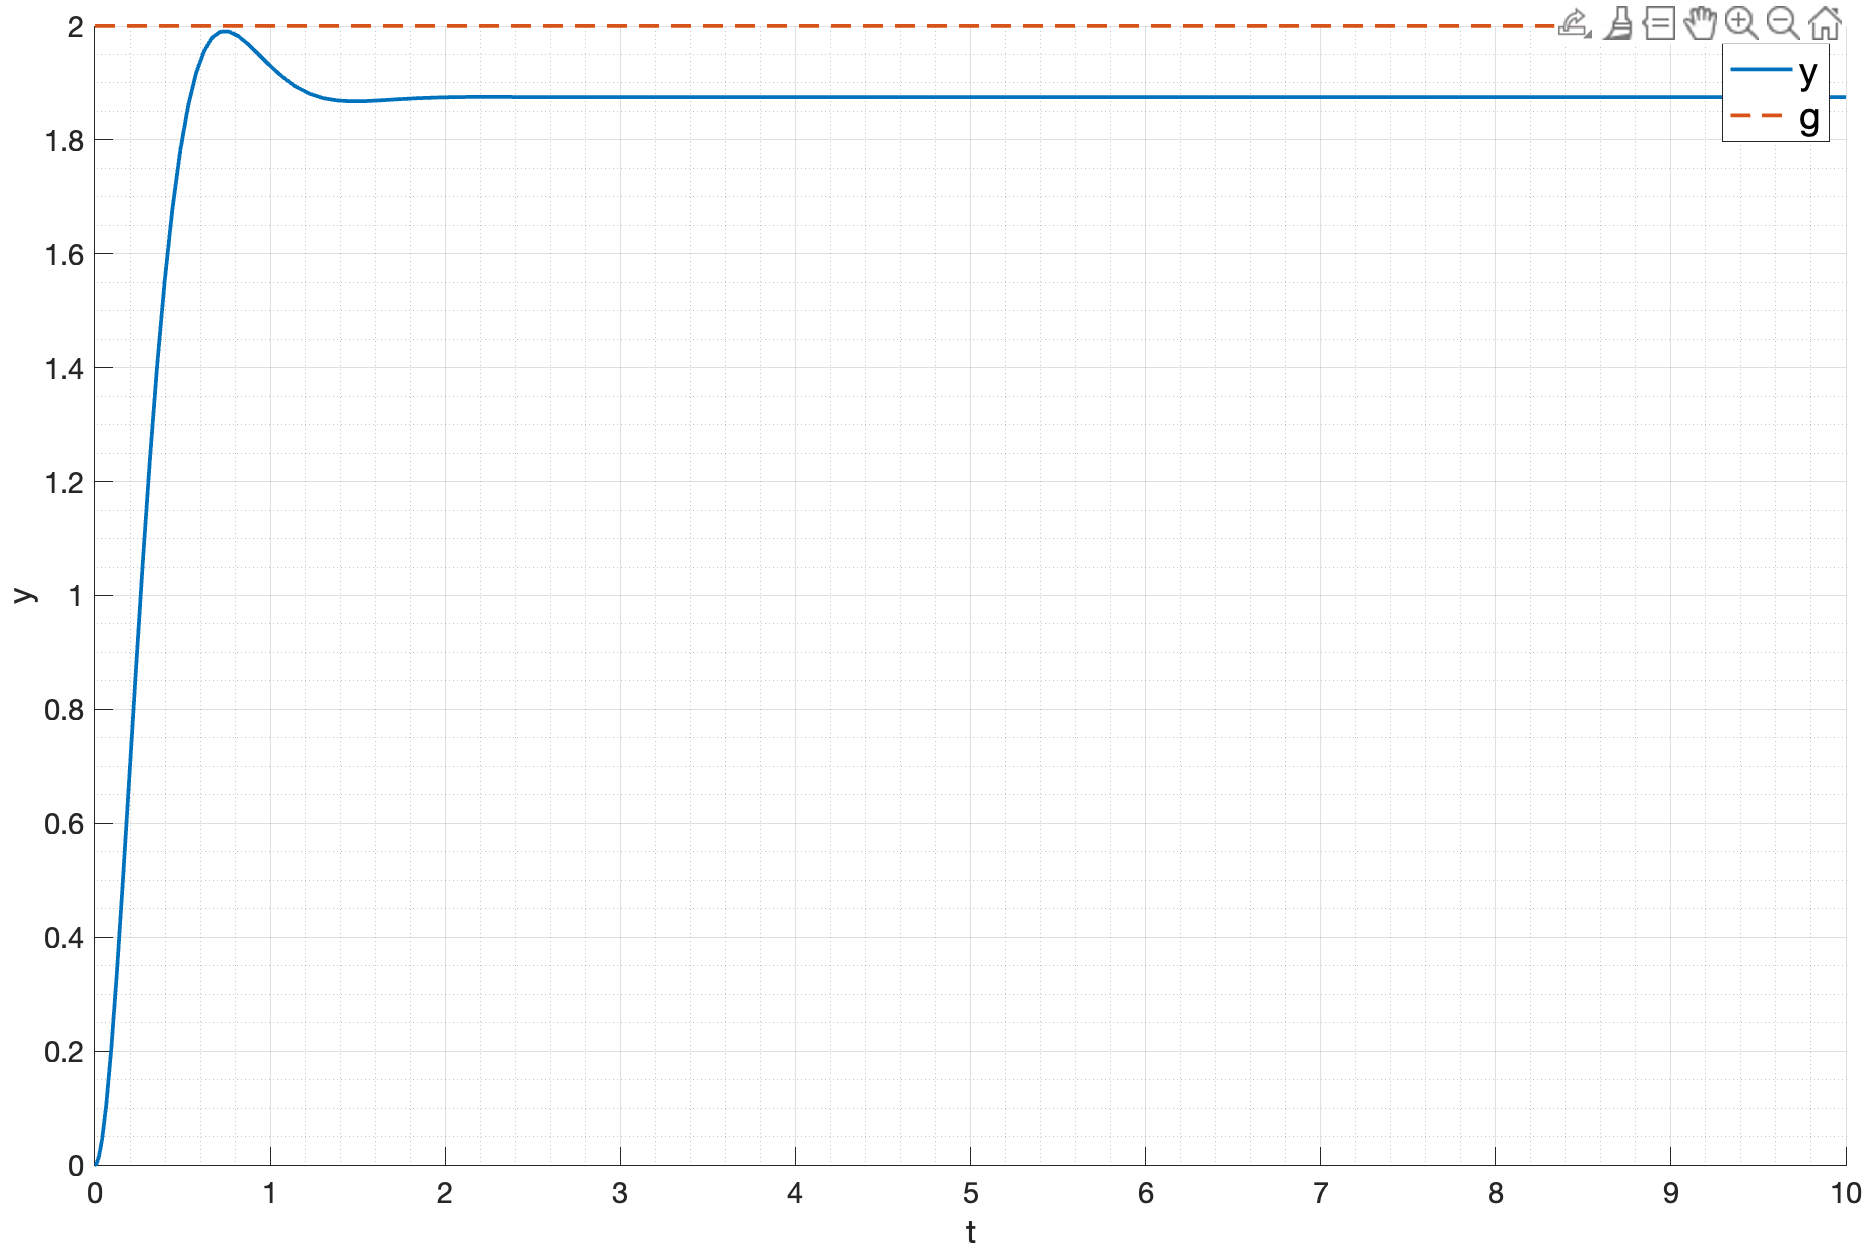
\includegraphics[width=\textwidth]{"media/plots/task3_out4.png"}
%     \caption{Моделирование системы с P регулятором ($k = 10$) ($u(t) = A$)}
%     \label{fig:task3_out4}
% \end{figure}
% Фактическое значение установившегося значения ошибки  $e_{\text{fact}} = 0.125$.

Во всех случаях фактическое значение установившегося значения ошибки совпадает с теоретическим, что 
подтверждает правильность выводов о стабильности системы и установившемся значении ошибки. 

\subsection{Система с линейно возрастающим входным воздействием}
Рассмотрим систему с линейно возрастающим входным воздействием:
\begin{equation}
    u(t) = Vt
\end{equation}
Найдем образ Лапласа входного воздействия:
\begin{equation}
    L\{u\} = \frac{V}{s^2}
\end{equation}
Найдем образ Лапласа выходного сигнала:
\begin{equation}
    Y = W_{u\rightarrow y}(s)L\{u\} = \frac{3k}{s^2 + 7.5s + 2 + 3k}\frac{V}{s^2} = \frac{3kV}{s^2(s^2 + 7.5s + 2 + 3k)}
\end{equation}
Значение $sY$ имеет нулевые полюса, следовательно, теорема о конечном значении не применима.

Проведем моделирование системы с линейно возрастающим входным воздействием. При тех же 
значениях $k$ (см. рис. \ref{fig:task3_out2}, \ref{fig:task3_error2}).

\begin{figure}
    \centering
    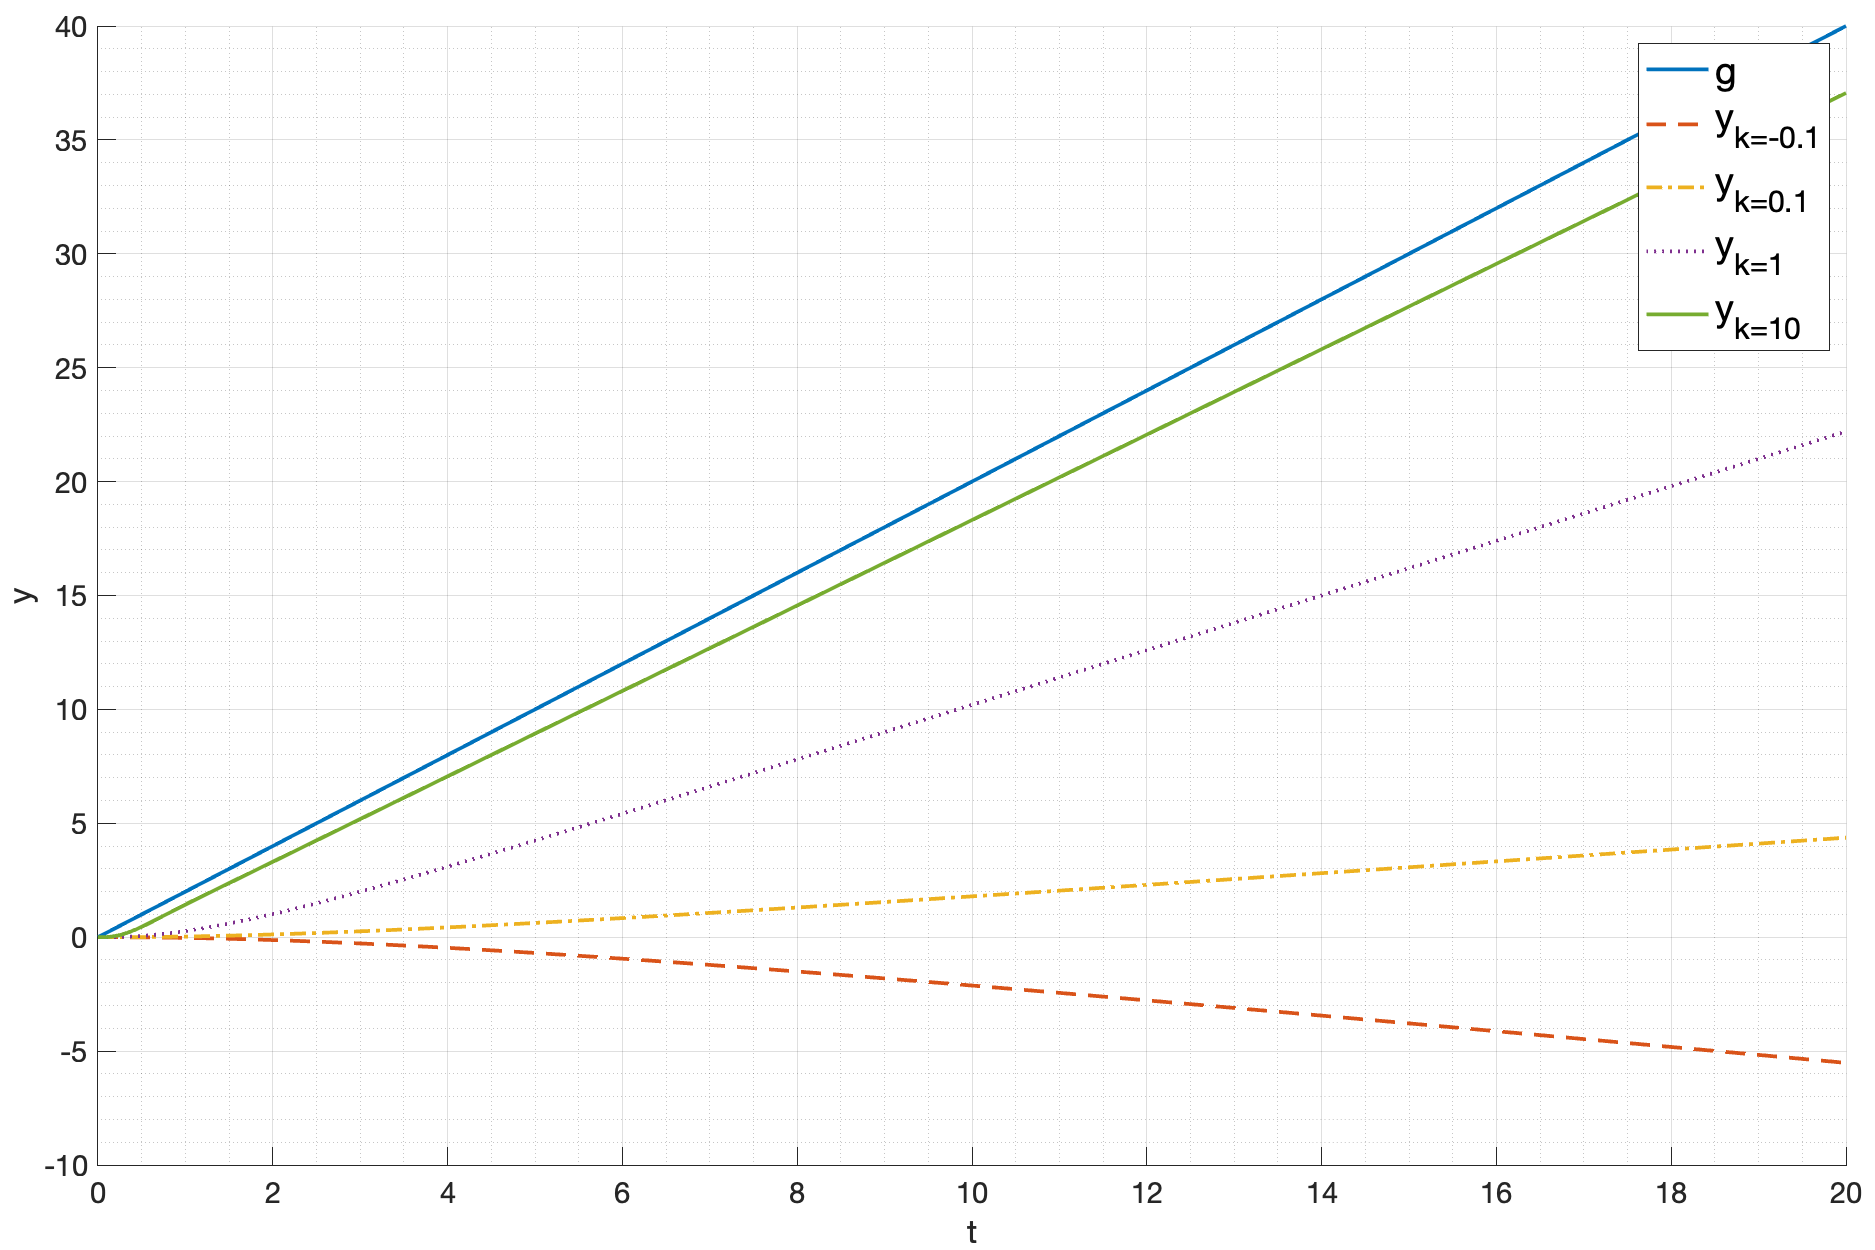
\includegraphics[width=\textwidth]{"media/plots/task3_out2.png"}
    \caption{Моделирование системы с P регулятором ($u(t) = Vt$)}
    \label{fig:task3_out2}
\end{figure}

\begin{figure}
    \centering
    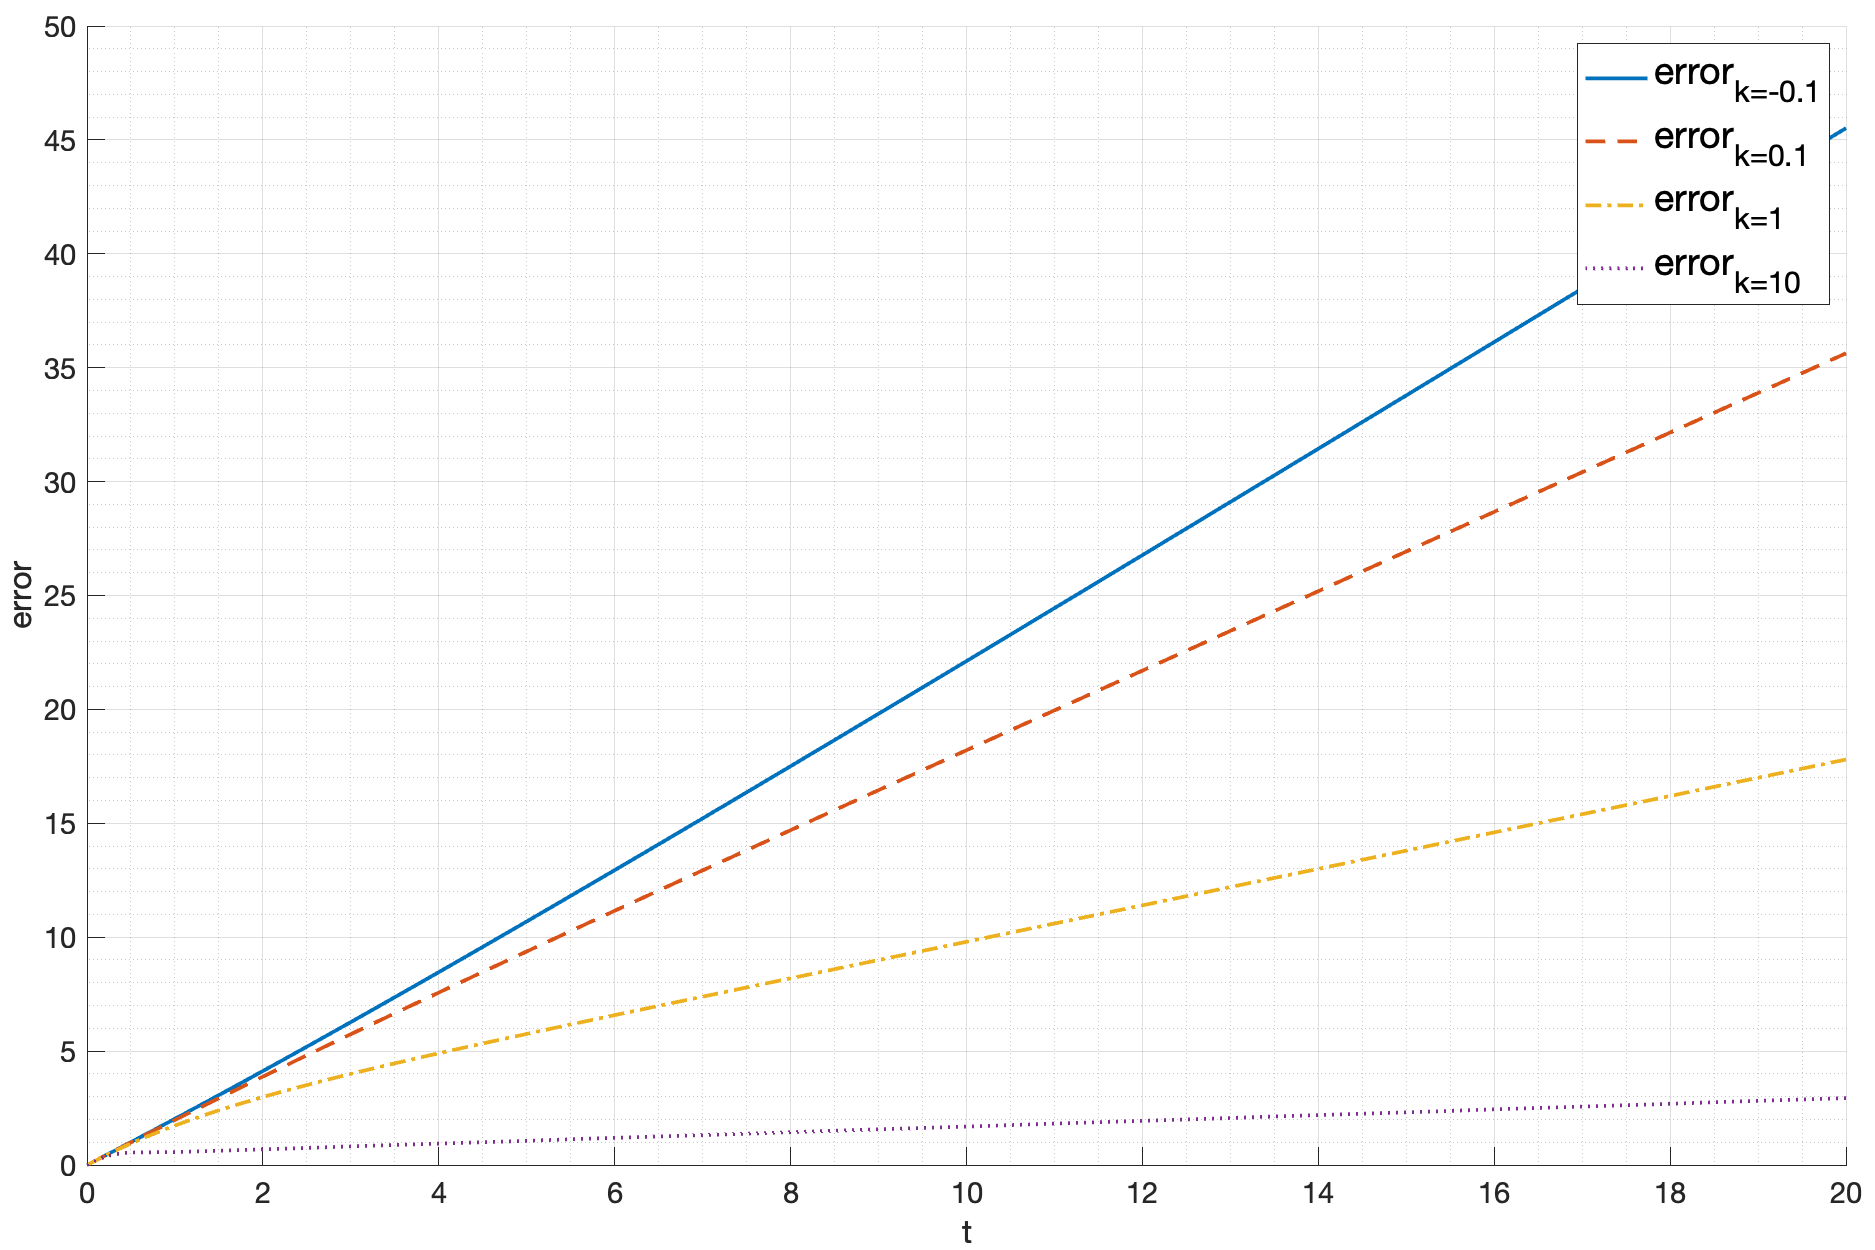
\includegraphics[width=\textwidth]{"media/plots/task3_error2.png"}
    \caption{График ошибки системы с P регулятором ($u(t) = Vt$)}
    \label{fig:task3_error2}
\end{figure}

% Проведем моделирование системы с линейно возрастающим входным воздействием. При тех же 
% значениях $k$ (см. рис. \ref{fig:task3_out5}, \ref{fig:task3_out6}, \ref{fig:task3_out7}, \ref{fig:task3_out8}).
% Графики ошибок приведены на рис. \ref{fig:task3_error5}, \ref{fig:task3_error6}, \ref{fig:task3_error7}, \ref{fig:task3_error8}.

% \begin{figure}
%     \centering
%     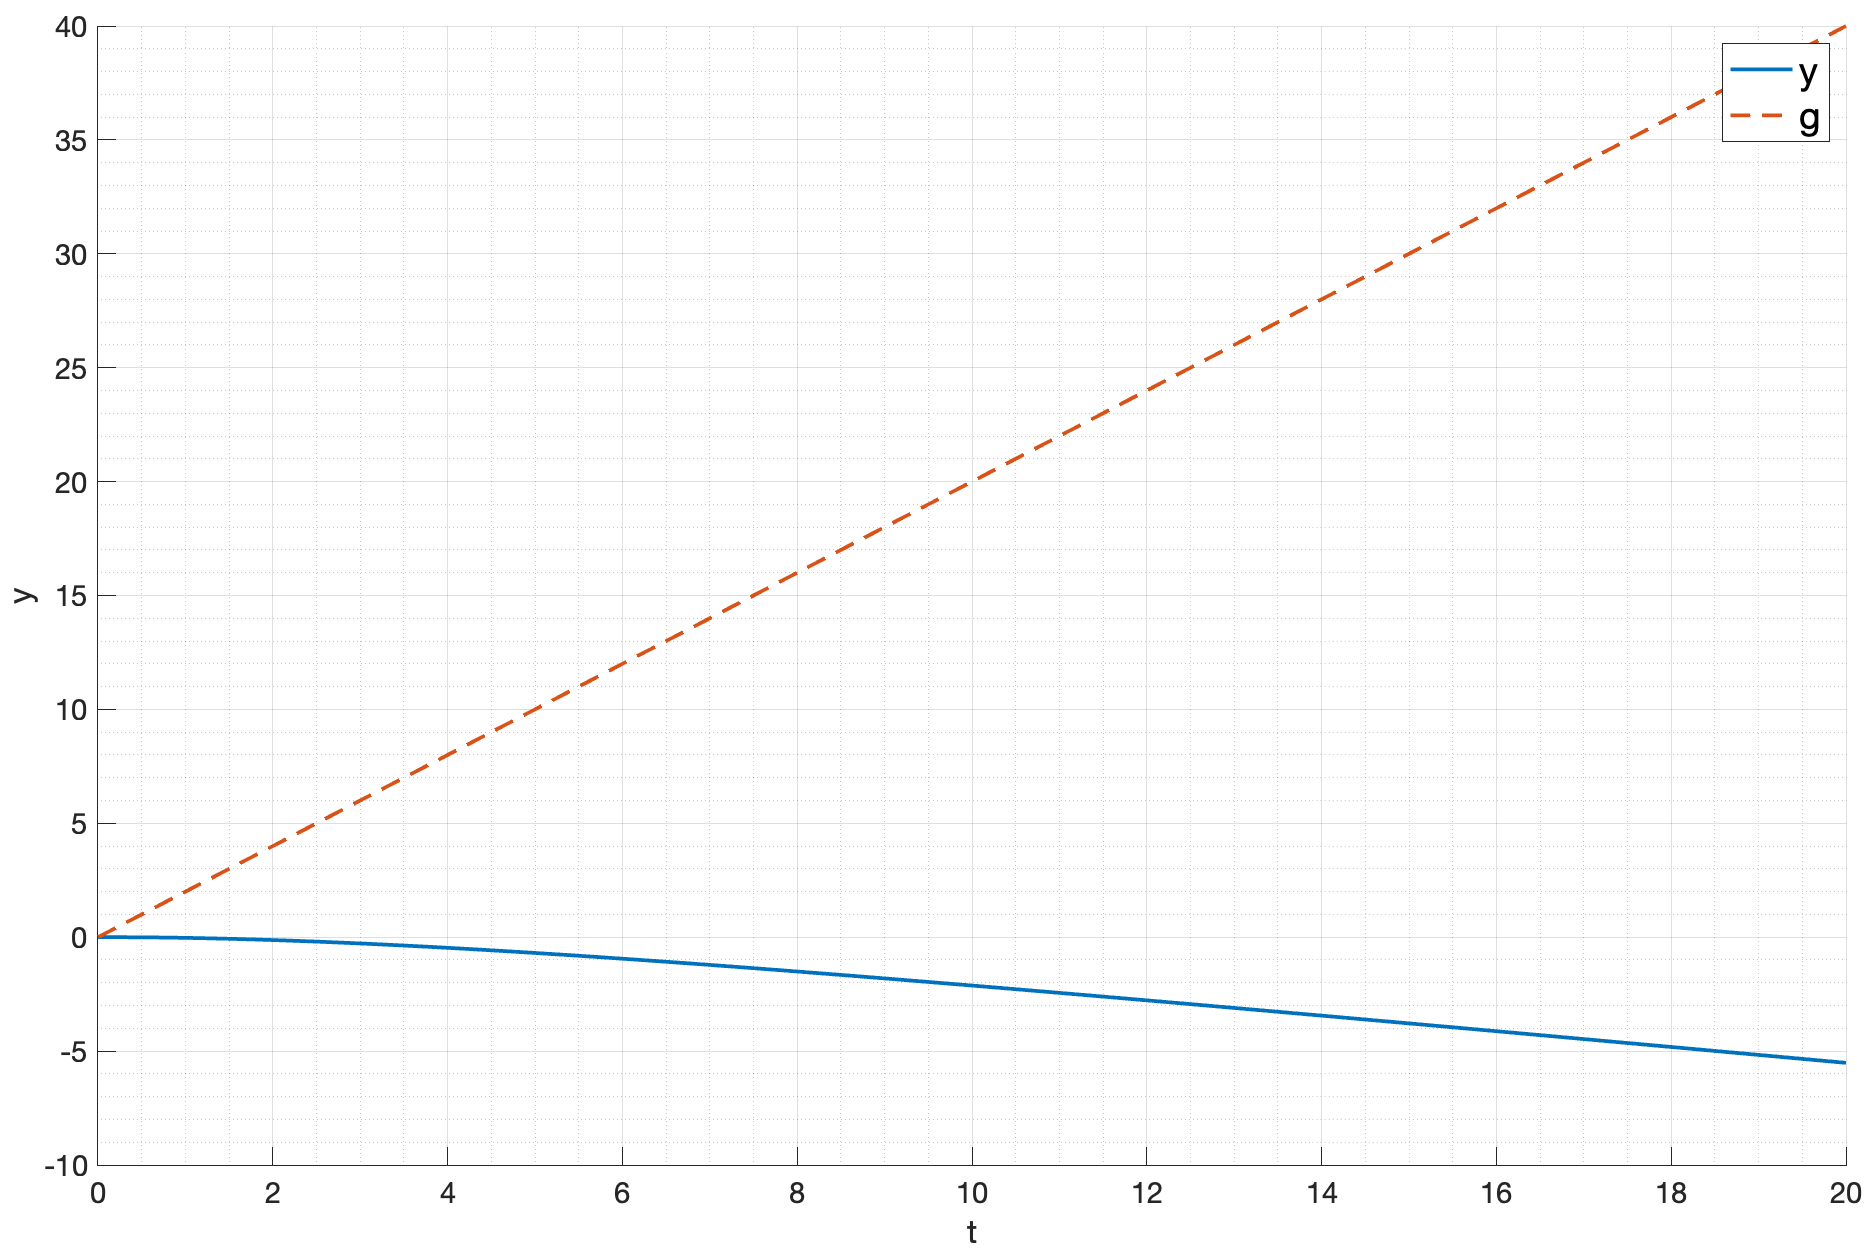
\includegraphics[width=\textwidth]{"media/plots/task3_out5.png"}
%     \caption{Моделирование системы с P регулятором ($k = -0.1$) ($u(t) = Vt$)}
%     \label{fig:task3_out5}
% \end{figure}

% \begin{figure}
%     \centering
%     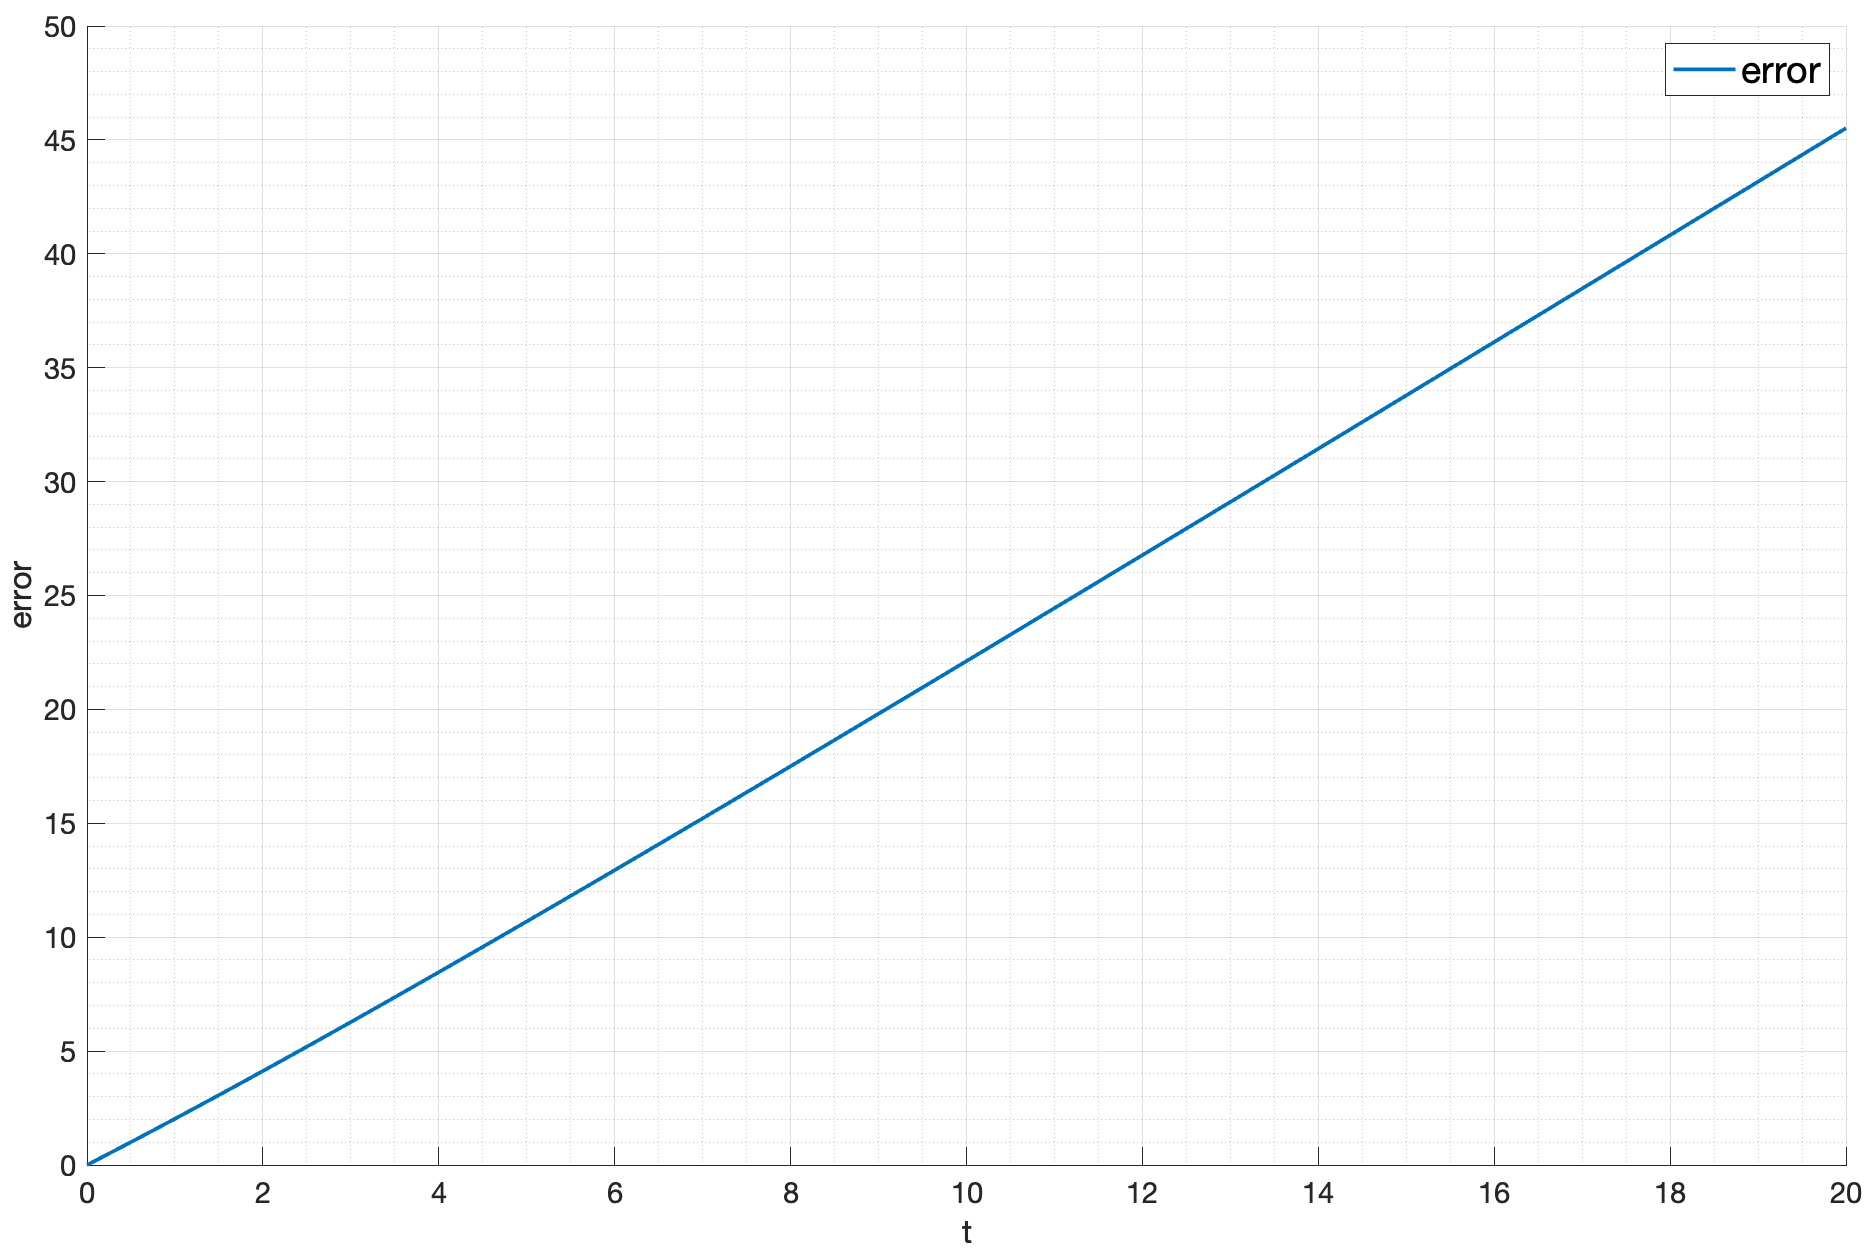
\includegraphics[width=\textwidth]{"media/plots/task3_error5.png"}
%     \caption{График ошибки системы с P регулятором ($k = -0.1$) ($u(t) = Vt$)}
%     \label{fig:task3_error5}
% \end{figure}

% \begin{figure}
%     \centering
%     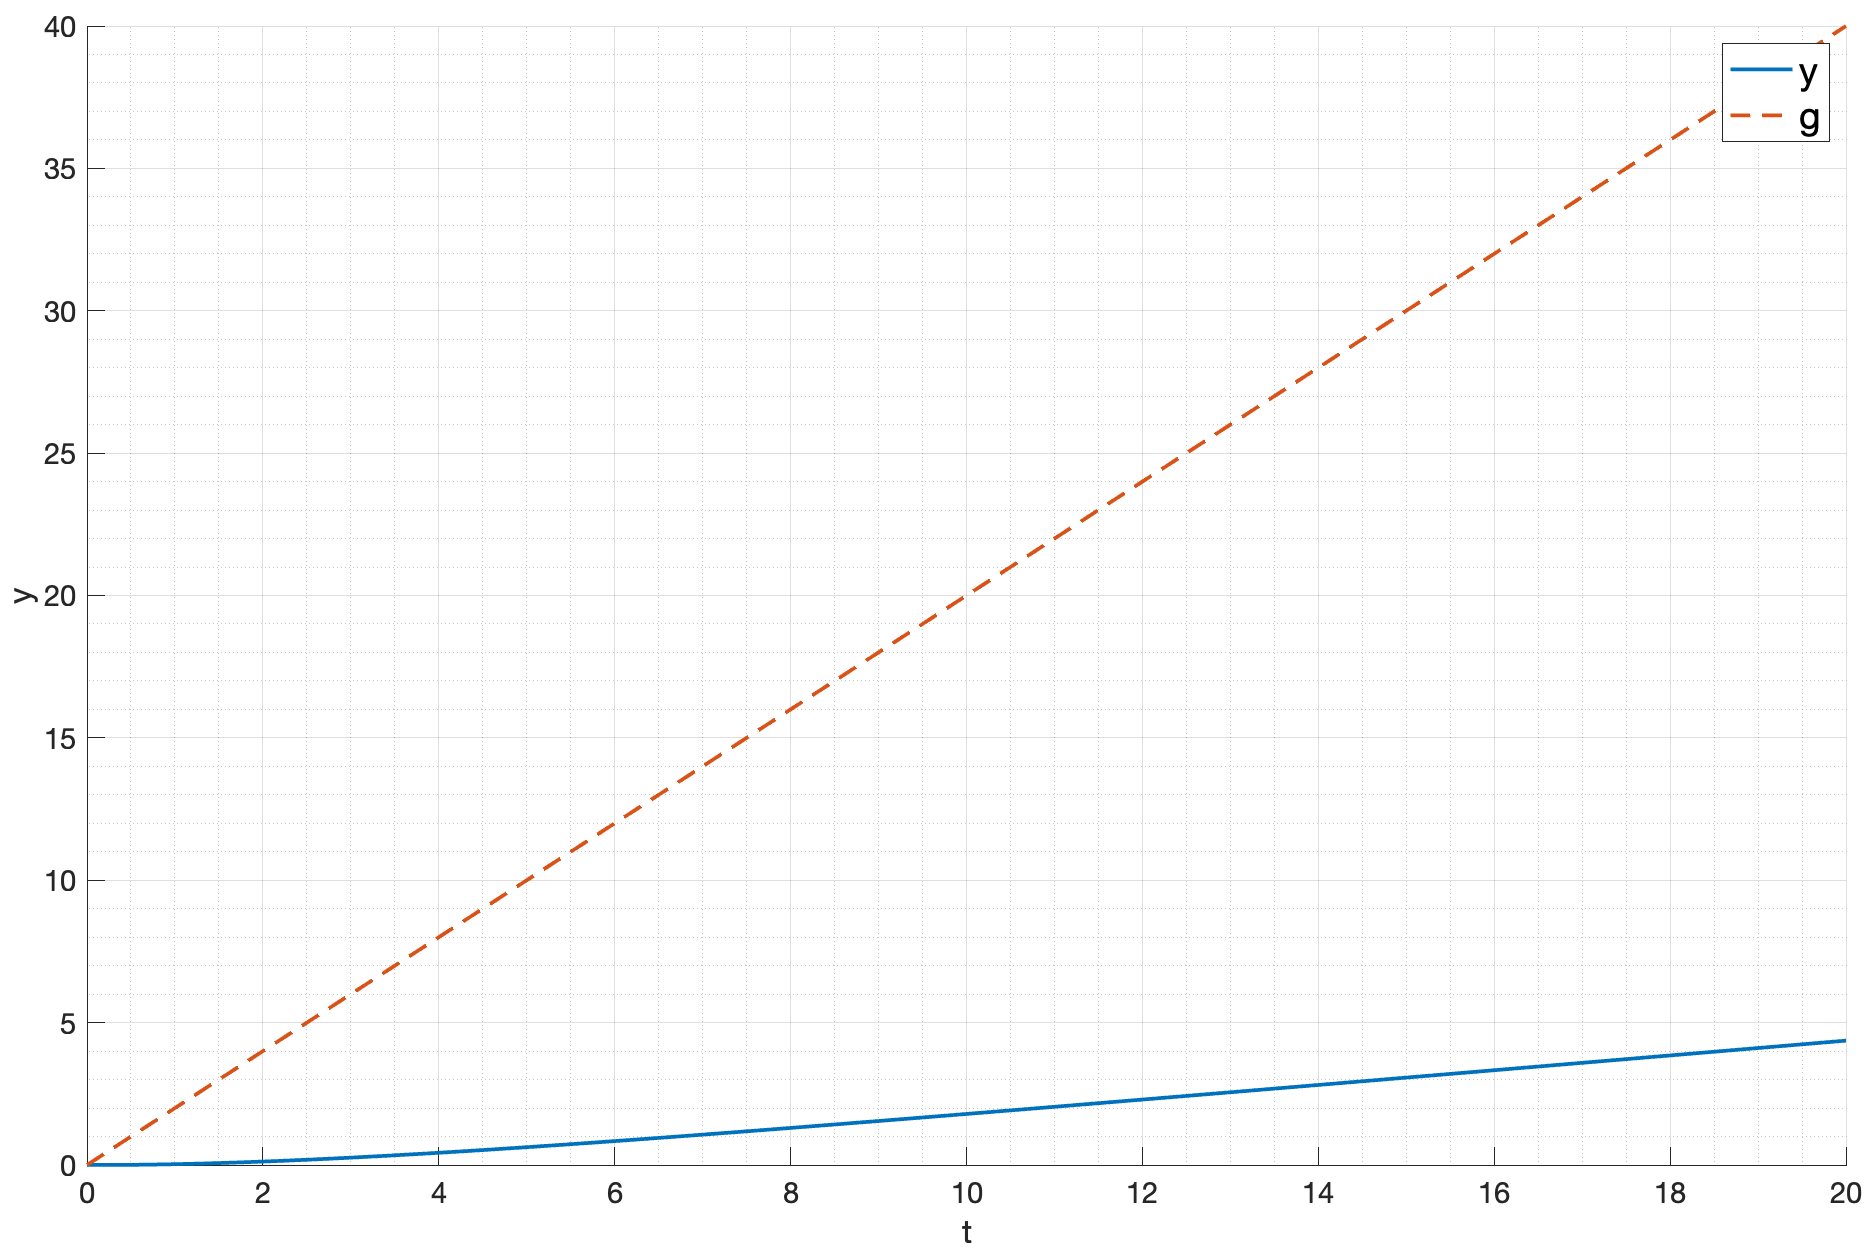
\includegraphics[width=\textwidth]{"media/plots/task3_out6.png"}
%     \caption{Моделирование системы с P регулятором ($k = 0.1$) ($u(t) = Vt$)}
%     \label{fig:task3_out6}
% \end{figure}

% \begin{figure}
%     \centering
%     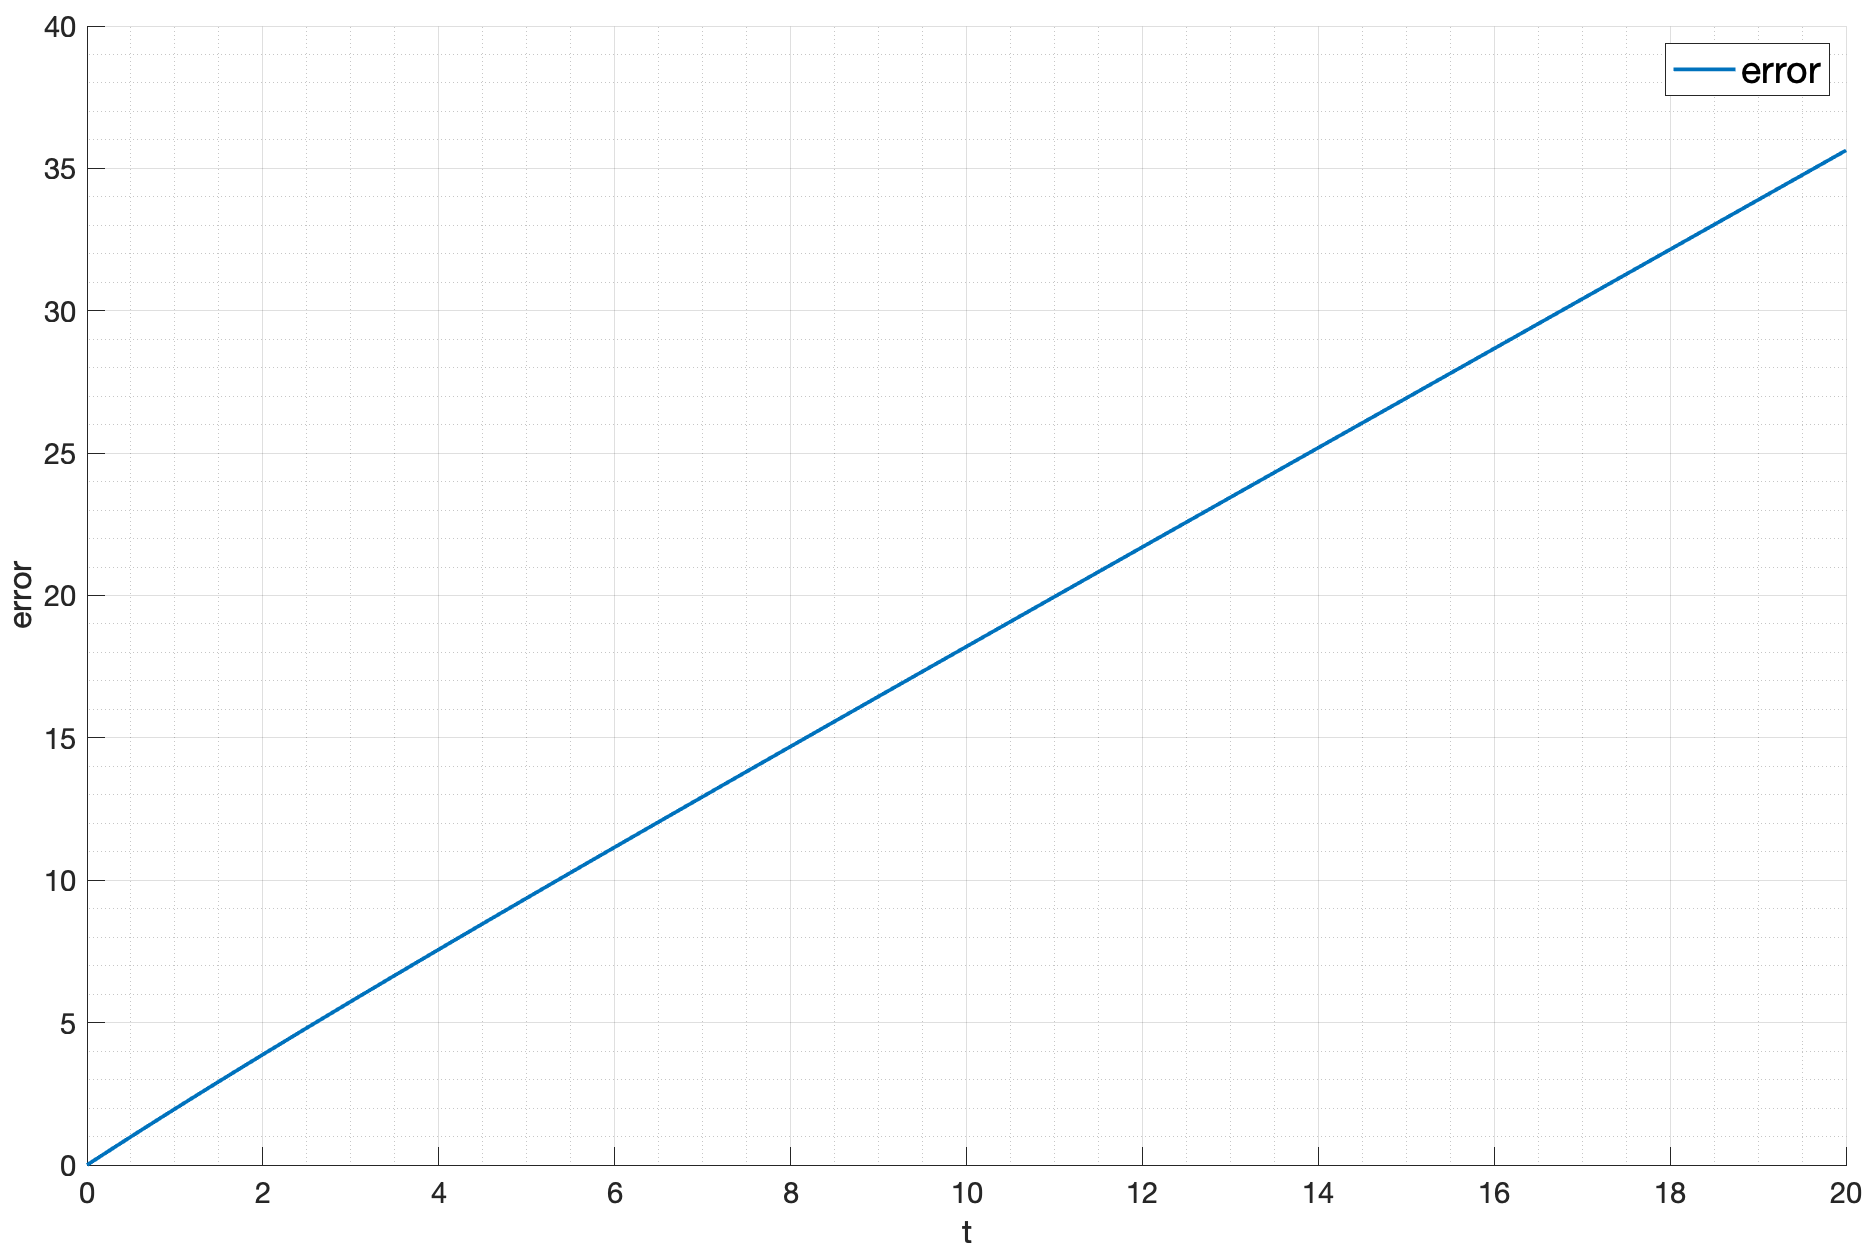
\includegraphics[width=\textwidth]{"media/plots/task3_error6.png"}
%     \caption{График ошибки системы с P регулятором ($k = 0.1$) ($u(t) = Vt$)}
%     \label{fig:task3_error6}
% \end{figure}


% \begin{figure}
%     \centering
%     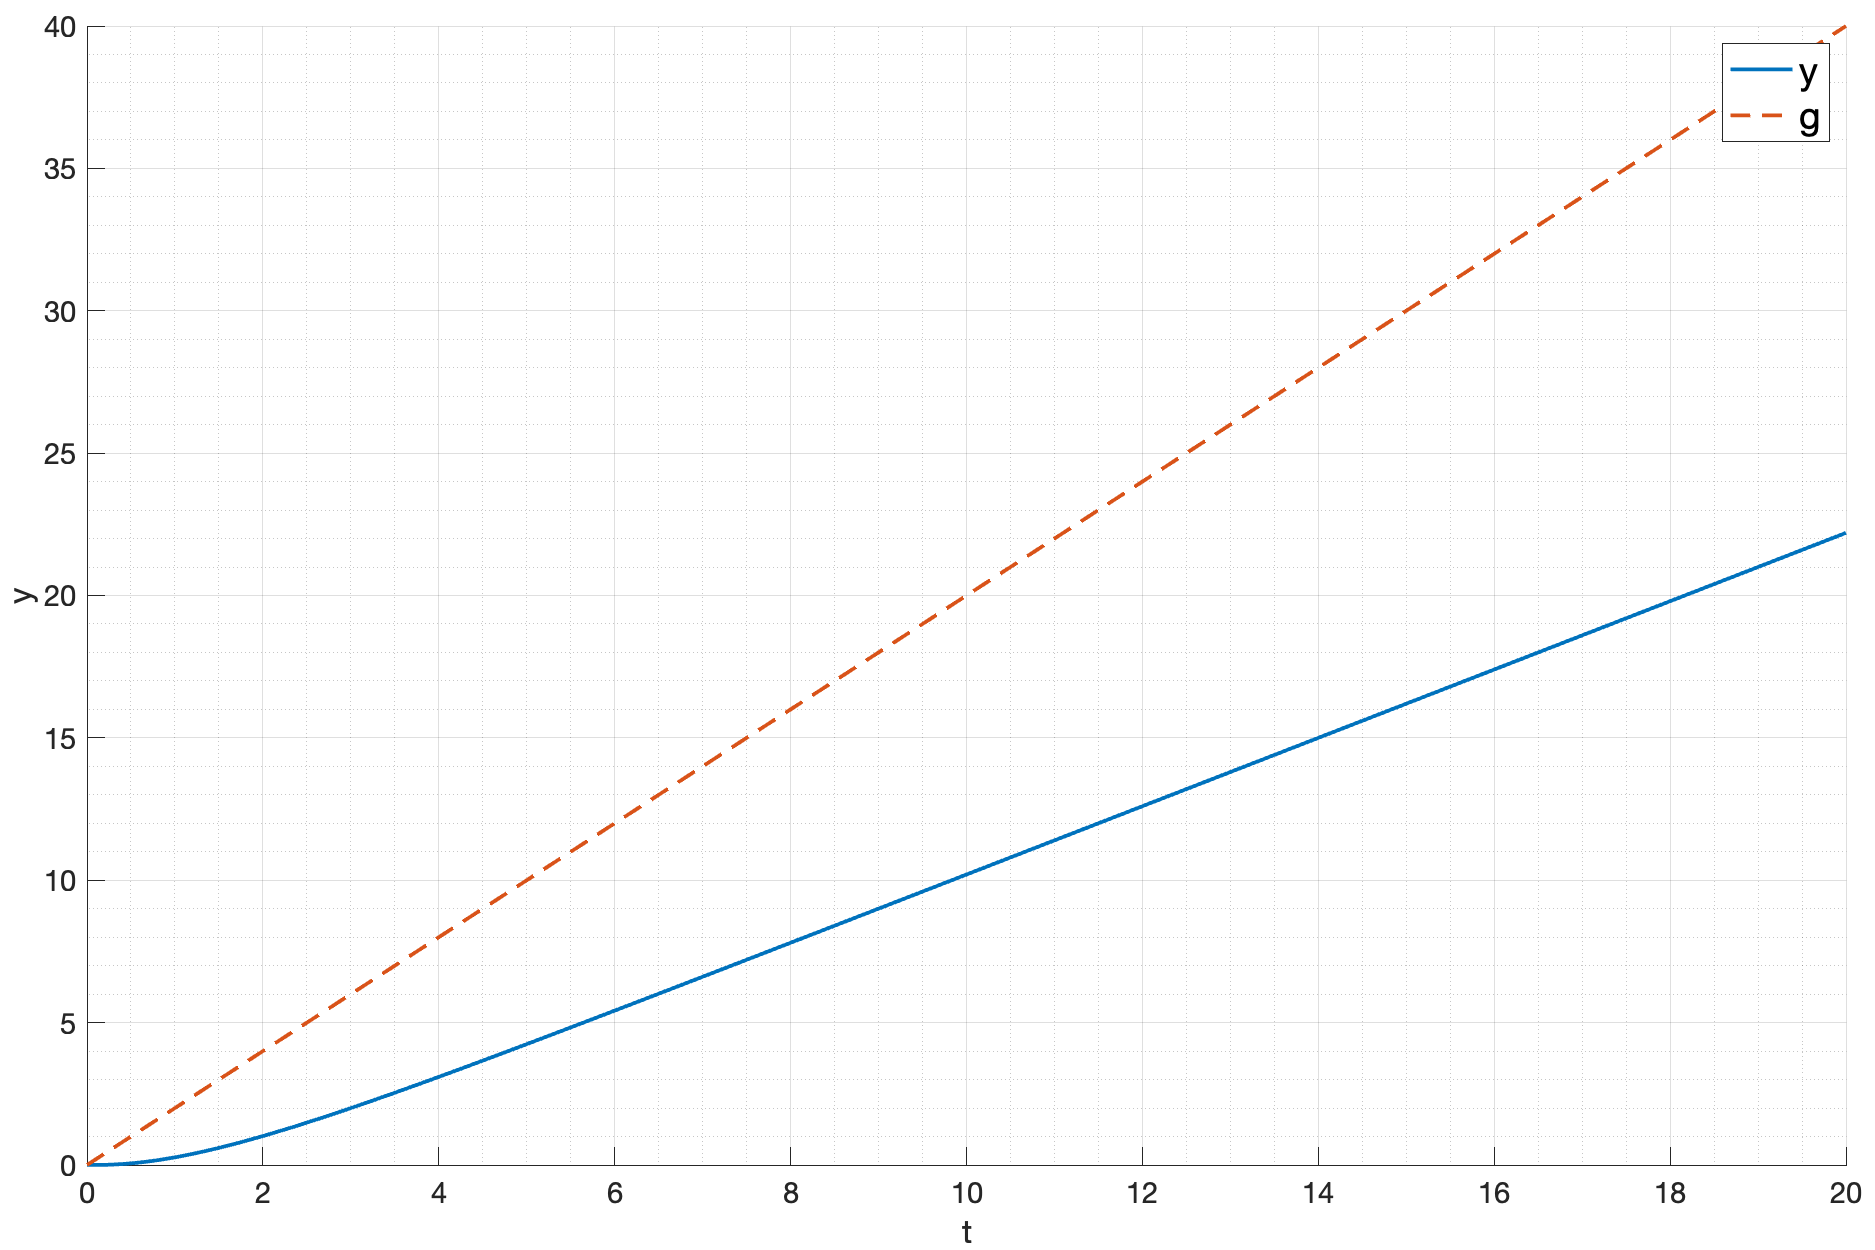
\includegraphics[width=\textwidth]{"media/plots/task3_out7.png"}
%     \caption{Моделирование системы с P регулятором ($k = 1$) ($u(t) = Vt$)}
%     \label{fig:task3_out7}
% \end{figure}

% \begin{figure}
%     \centering
%     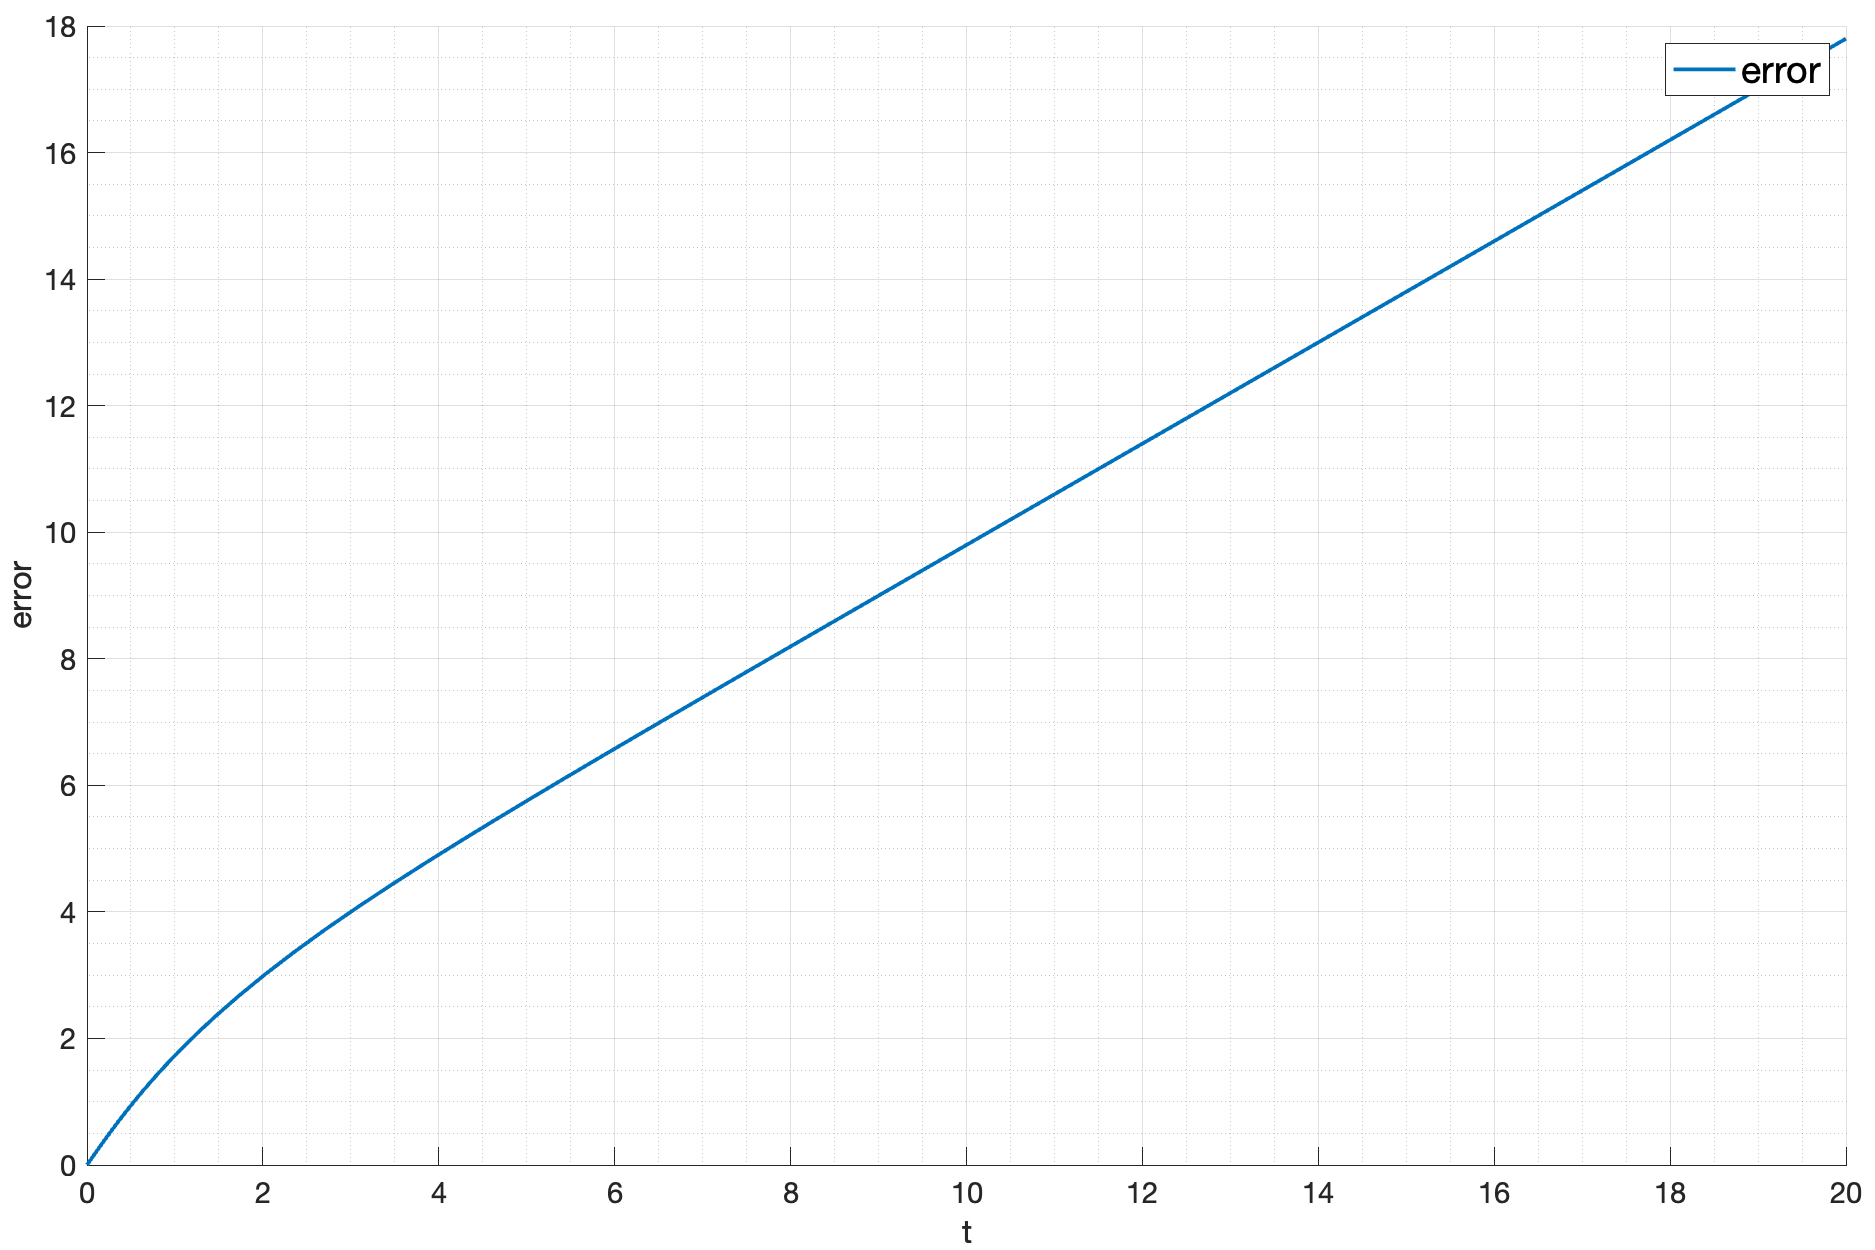
\includegraphics[width=\textwidth]{"media/plots/task3_error7.png"}
%     \caption{График ошибки системы с P регулятором ($k = 1$) ($u(t) = Vt$)}
%     \label{fig:task3_error7}
% \end{figure}

% \begin{figure}
%     \centering
%     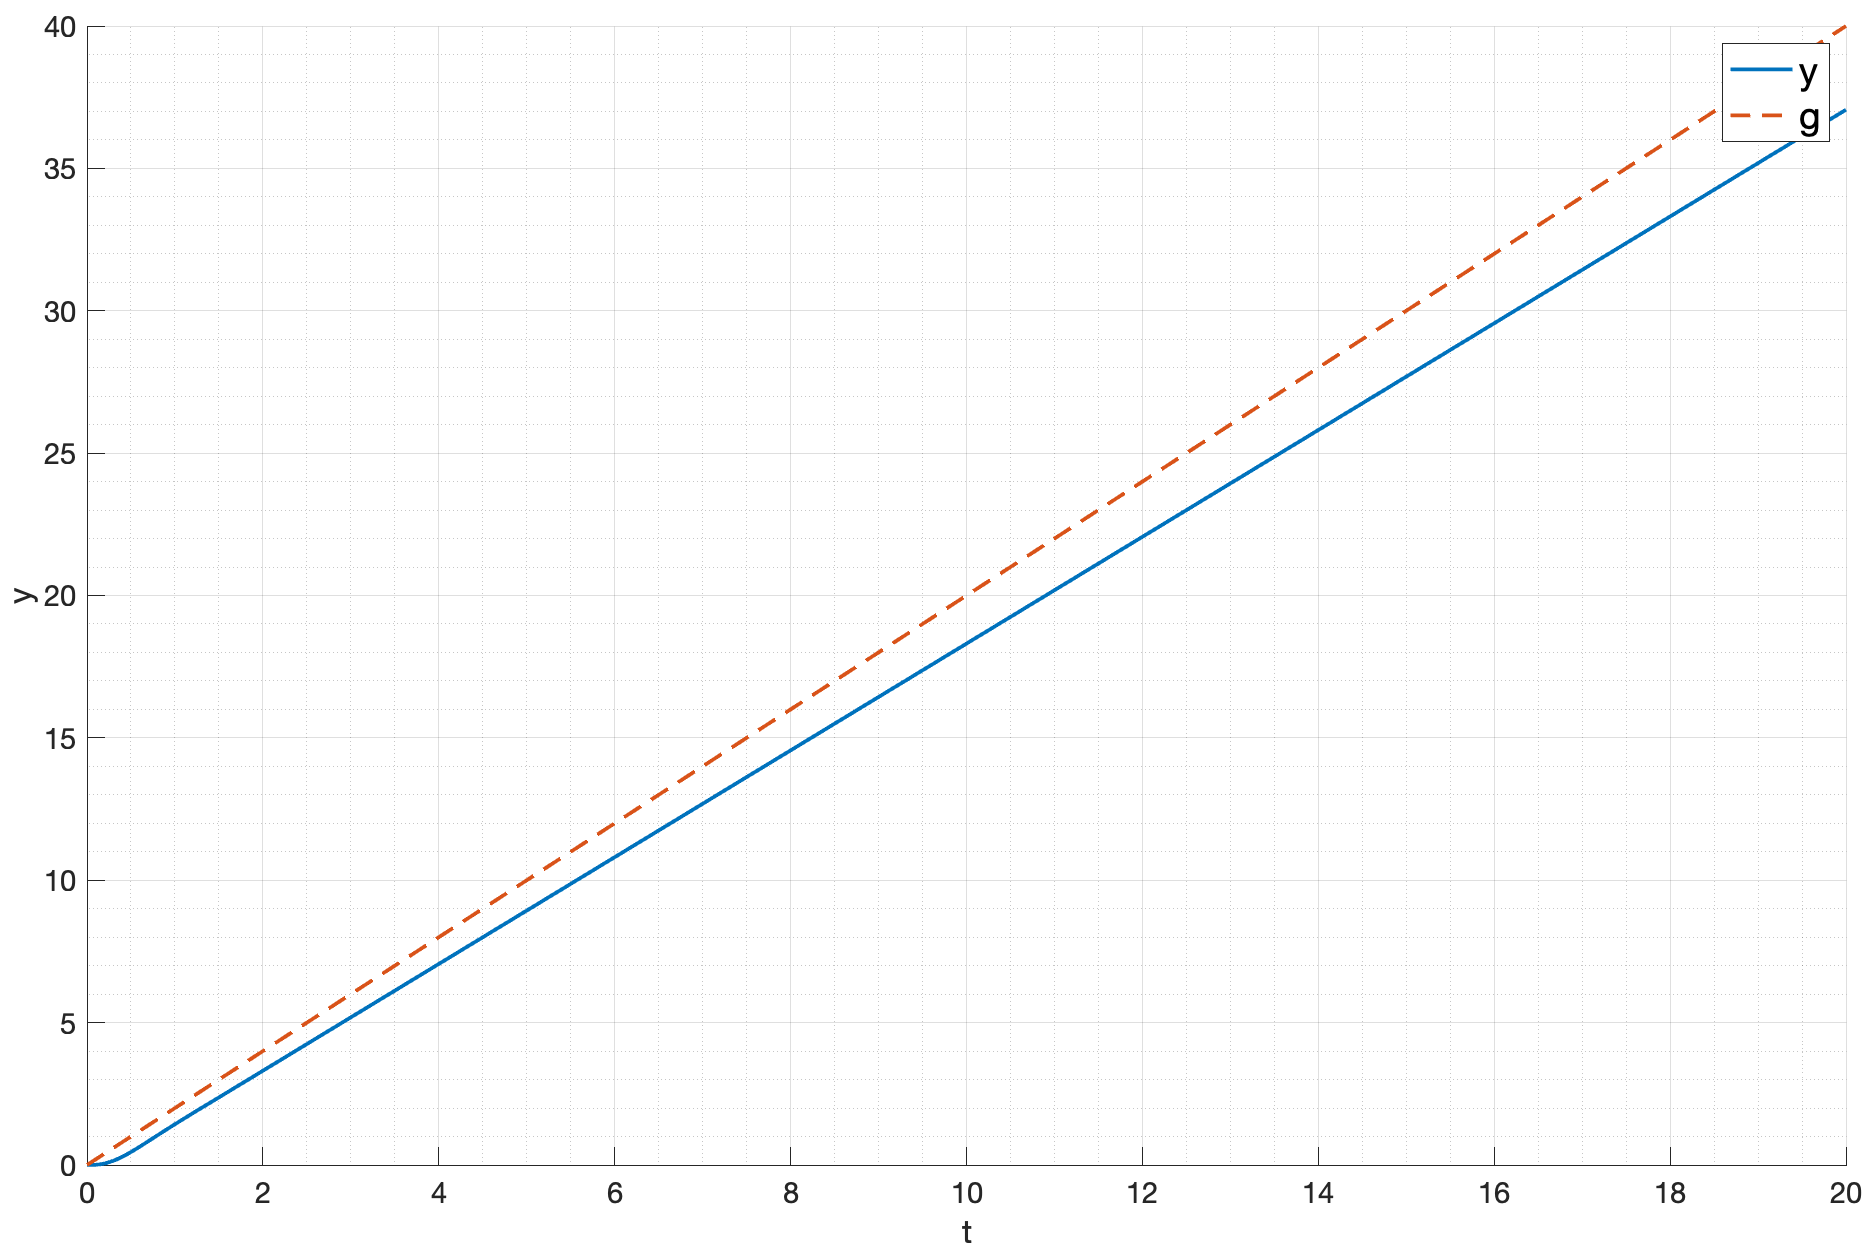
\includegraphics[width=\textwidth]{"media/plots/task3_out8.png"}
%     \caption{Моделирование системы с P регулятором ($k = 10$) ($u(t) = Vt$)}
%     \label{fig:task3_out8}
% \end{figure}

% \begin{figure}
%     \centering
%     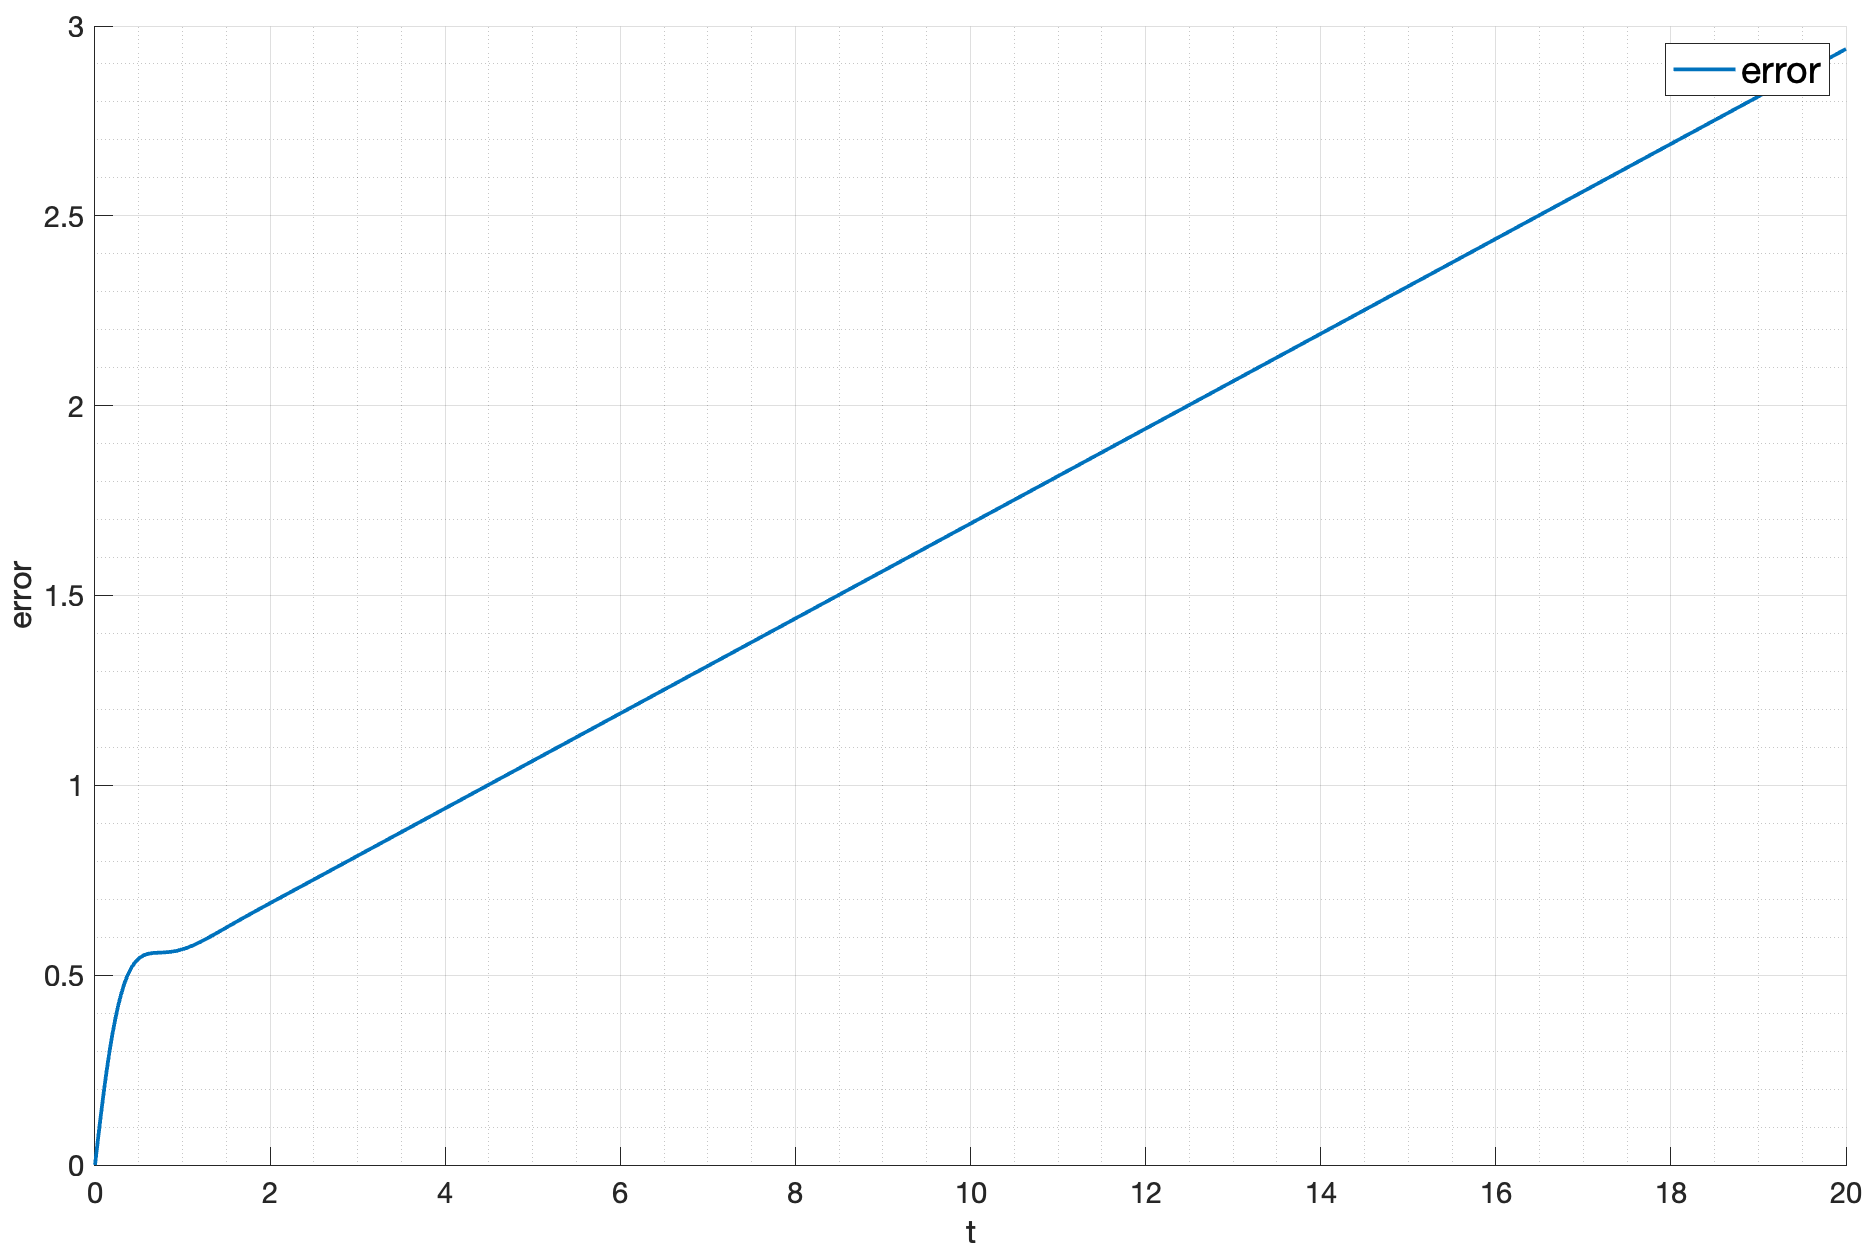
\includegraphics[width=\textwidth]{"media/plots/task3_error8.png"}
%     \caption{График ошибки системы с P регулятором ($k = 10$) ($u(t) = Vt$)}
%     \label{fig:task3_error8}
% \end{figure}

Видно, что при линейно возрастающем входном воздействии система не приходит к установившемуся значению, 
что подтверждает то, что система является астатической нулевого порядка. 
\FloatBarrier
\subsection{Вывод}
В данном пункте была рассмотрена система с астатизмом нулевого порядка и P регулятором,
влияние коэффициента $k$ на систему. Была найдена область устойчивости системы и установившееся значение ошибки 
или показано, что система не будет приходить к установившемуся значению при линейно возрастающем входном воздействии.